\section{Eje X}
	\subsection{Material necesario}
		\begin{itemize}
			\item 3x tornillos M3x10.
			\item 1x tornillo M3x15. (recomendables M4)
			\item 1x tornillo M3x25. (recomendable M4)
			\item 1x tornillo M3x35. (recomendable M4)
			\item 3x tuertcas M3.
			\item 3x Arandelas M3.
			\item 1x polea mecanizada T2.5
			\item 1x Tornillo M8x40.
			\item 2x arandelas M8.
			\item 5x tuercas M8.
			\item 1x rodamientos axiales 608 zz blindados.
			\item 7x rodamientos lineales LM8UU.
			\item 2x varillas lisas M8x330.
			\item Bridas.
			\item Correa T2.5 de 720mm
			\item piezas X- motor, X idler, X carriege, Xtruder Mount.
		\end{itemize}
		\begin{figure}[!htp]
			\centering
			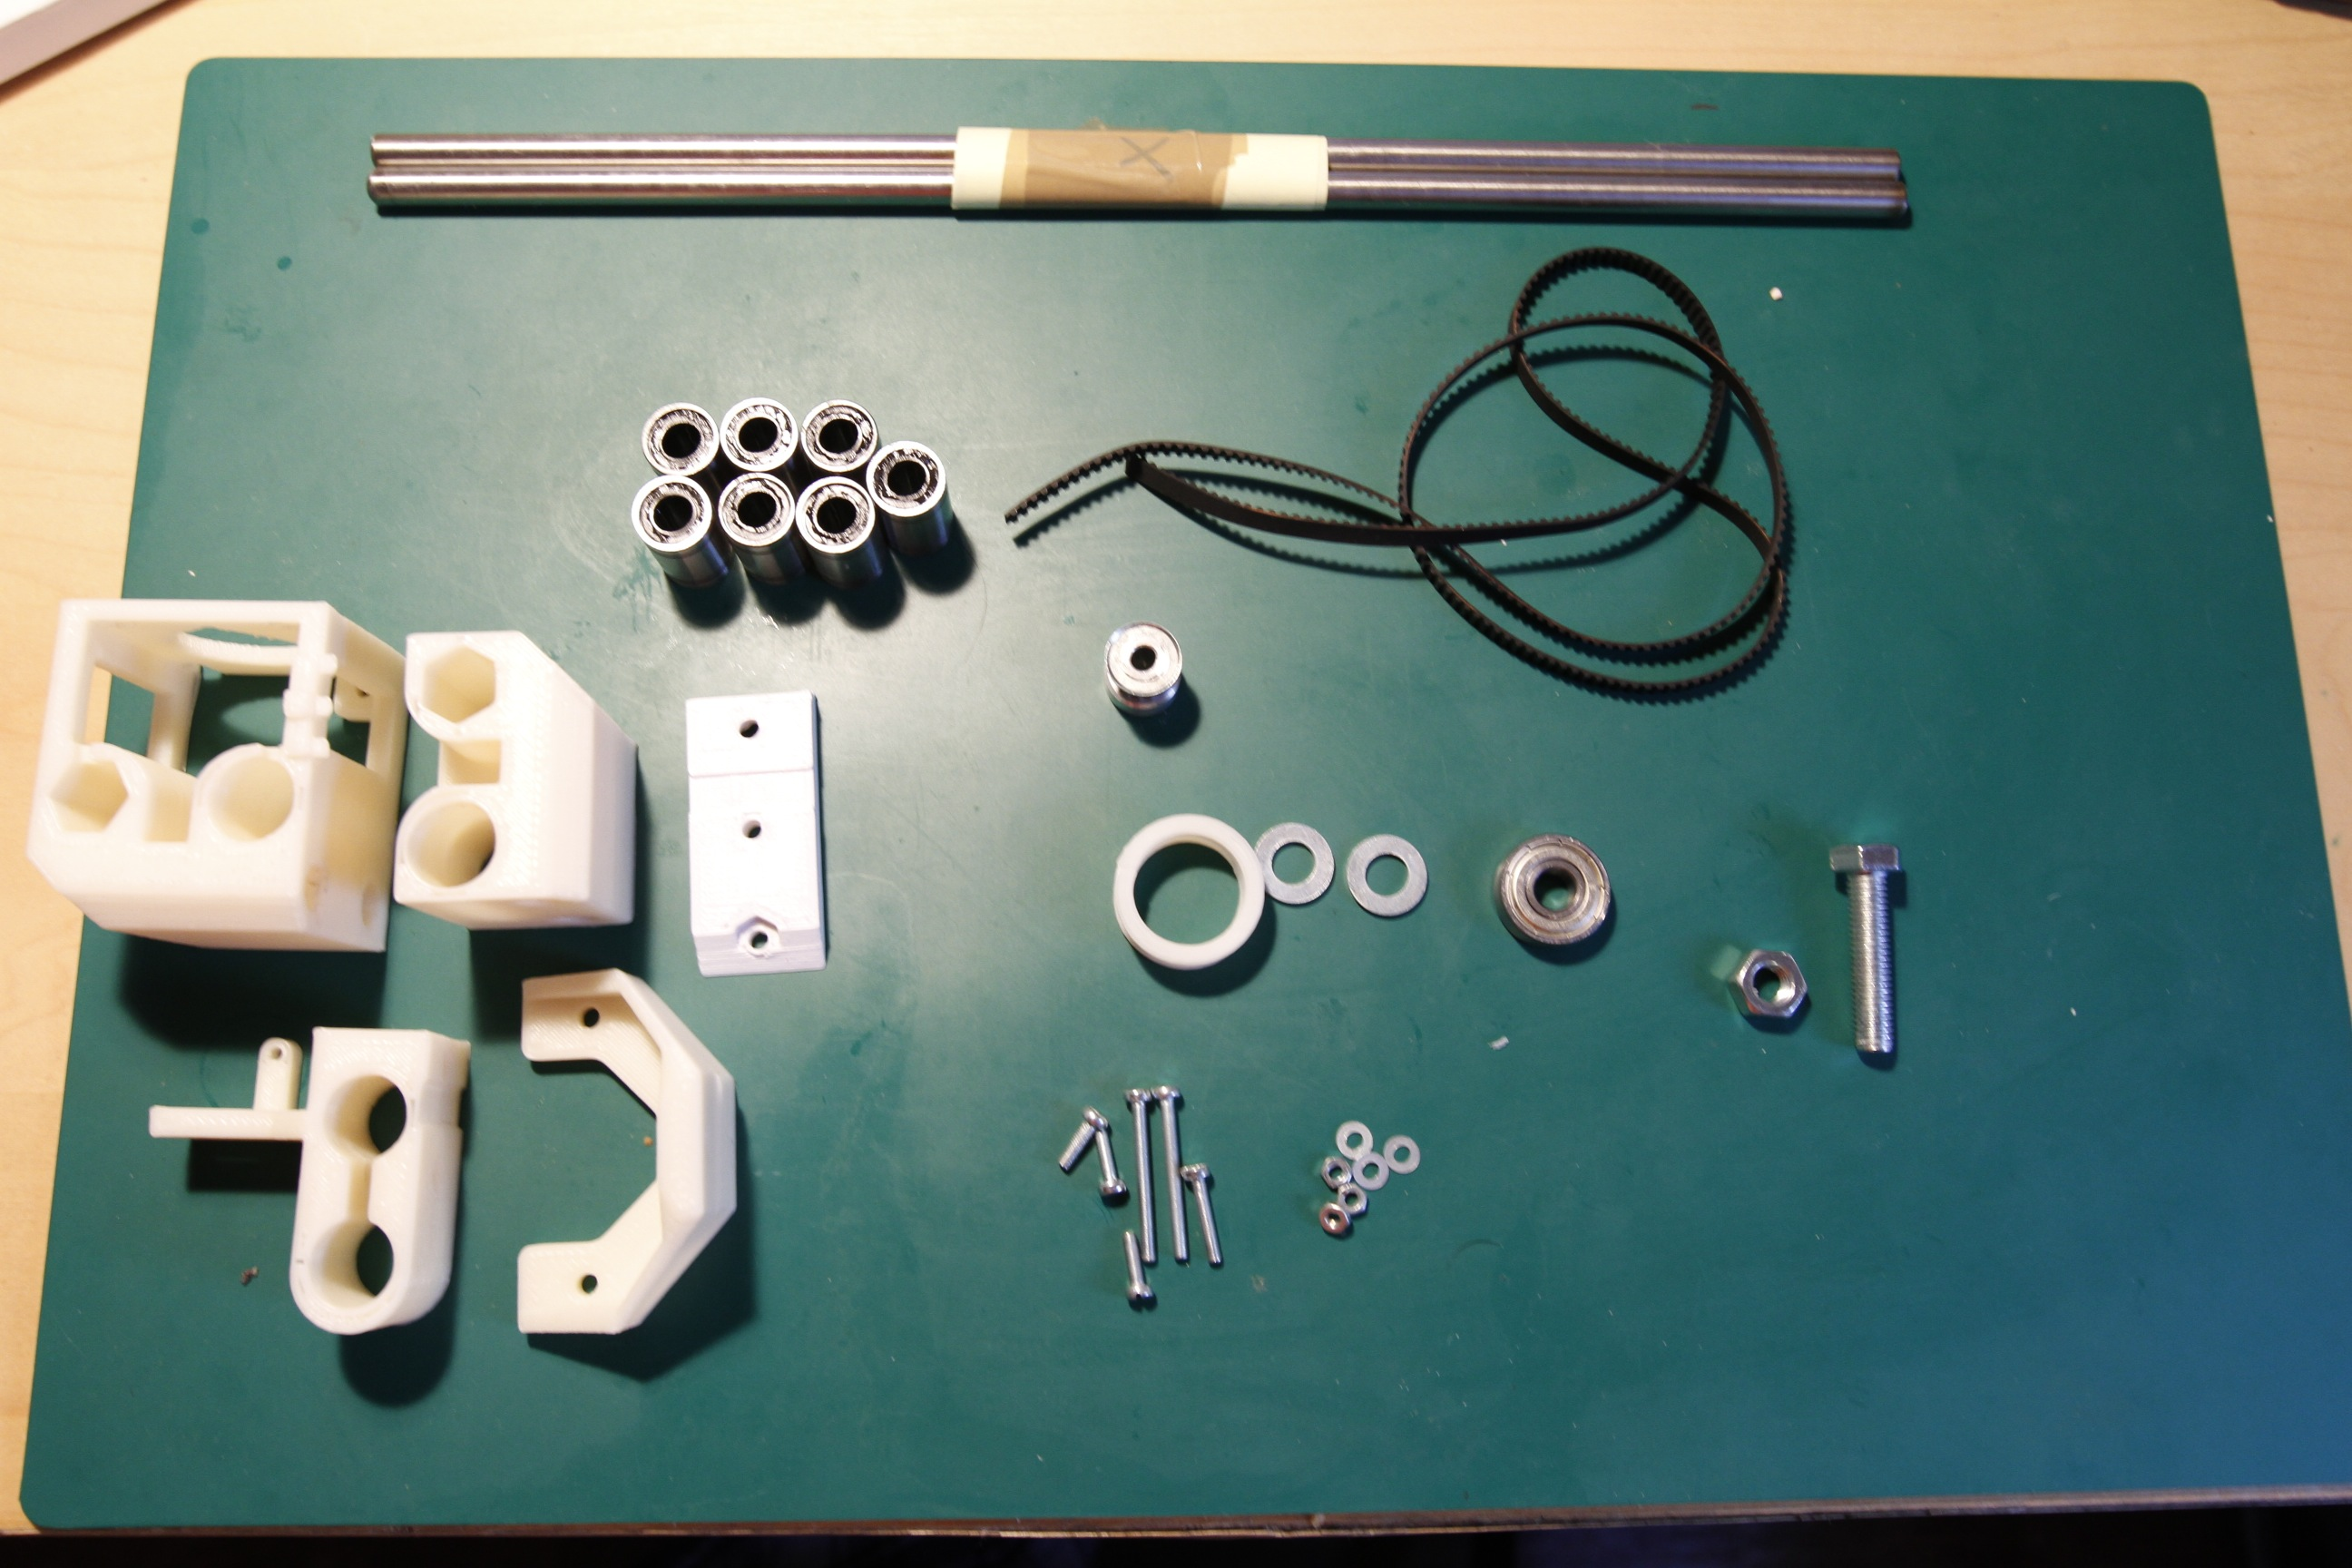
\includegraphics[width=0.6\textwidth]{../../Fotos/46.jpg}
			\caption{Material necesario}
		\end{figure}
		\newpage{}
	\subsection{Herramienta necesaria}
		\begin{itemize}
			\item Alicates de punta fina.
			\item Alicates de corte.
			\item Destornillador.
			\item limas.
			\item cutter
		\end{itemize}
		\begin{figure}[!htp]
			\centering
			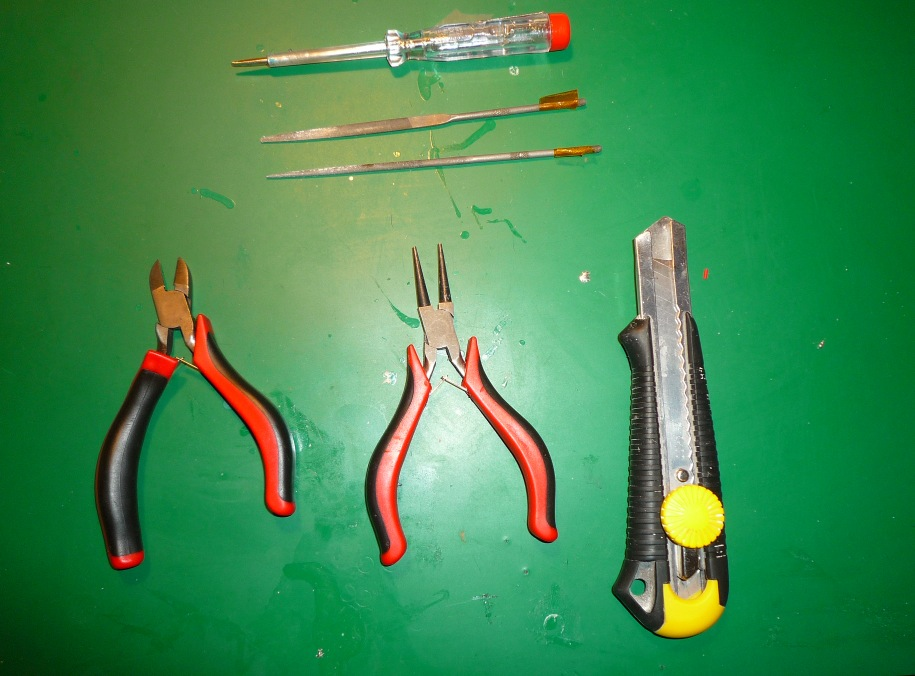
\includegraphics[width=0.6\textwidth]{../../Fotos/47.jpg}
			\caption{Herramienta necesaria}
		\end{figure}
	\newpage{}
	\subsection{Operativa}
		Lo primero que haremos será hacer el agujero pasante en la pieza X idler, a la hora de imprimir la pieza se tapa el agujero para poder hacer la pieza de una forma más sencilla. Para ellos nos ayudaremos de un cutter y una lima para hacerlo totalmente pasante ( Ver figura ~\ref{fig:agujero.pasante})\\
			\begin{figure}[H]
			        \centering
			        \begin{subfigure}[htb]{0.4\textwidth}
			                \centering
			                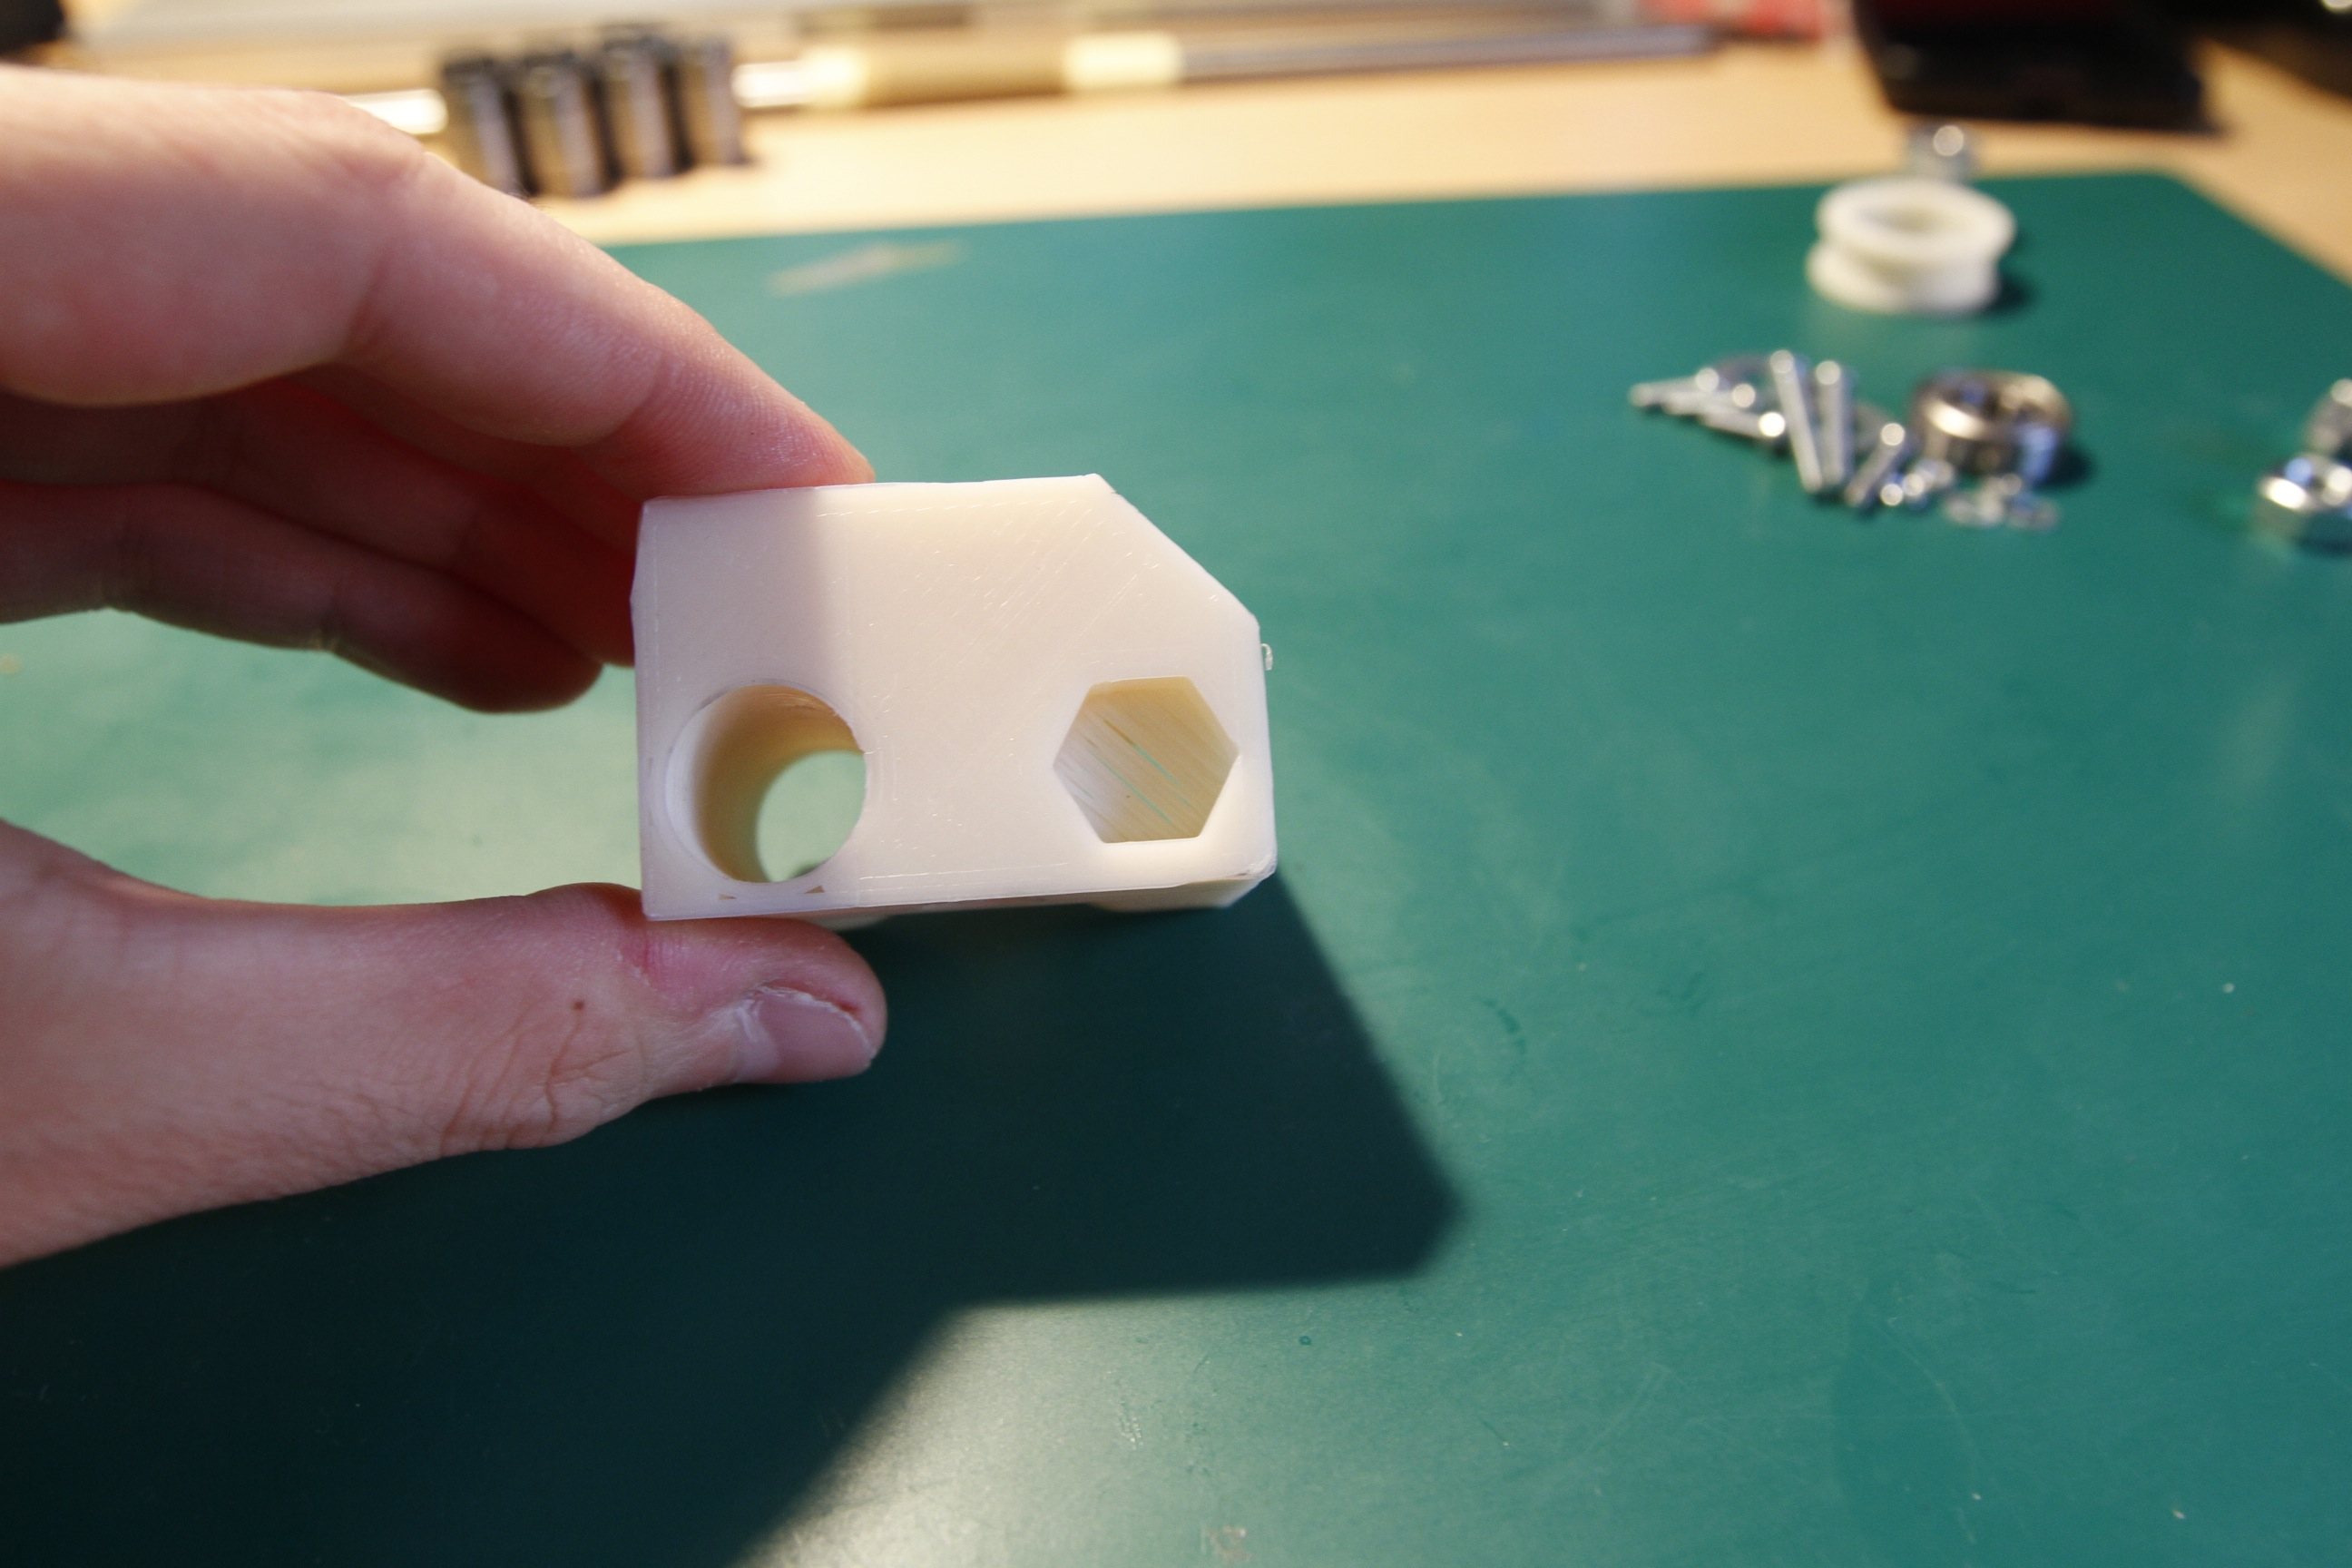
\includegraphics[width=\textwidth]{../../Fotos/48.jpg}
			                \caption{Agujero tapado }
			                \label{fig:agujero.tapado}
			        \end{subfigure}
			        \begin{subfigure}[htb]{0.4\textwidth}
			                \centering
			                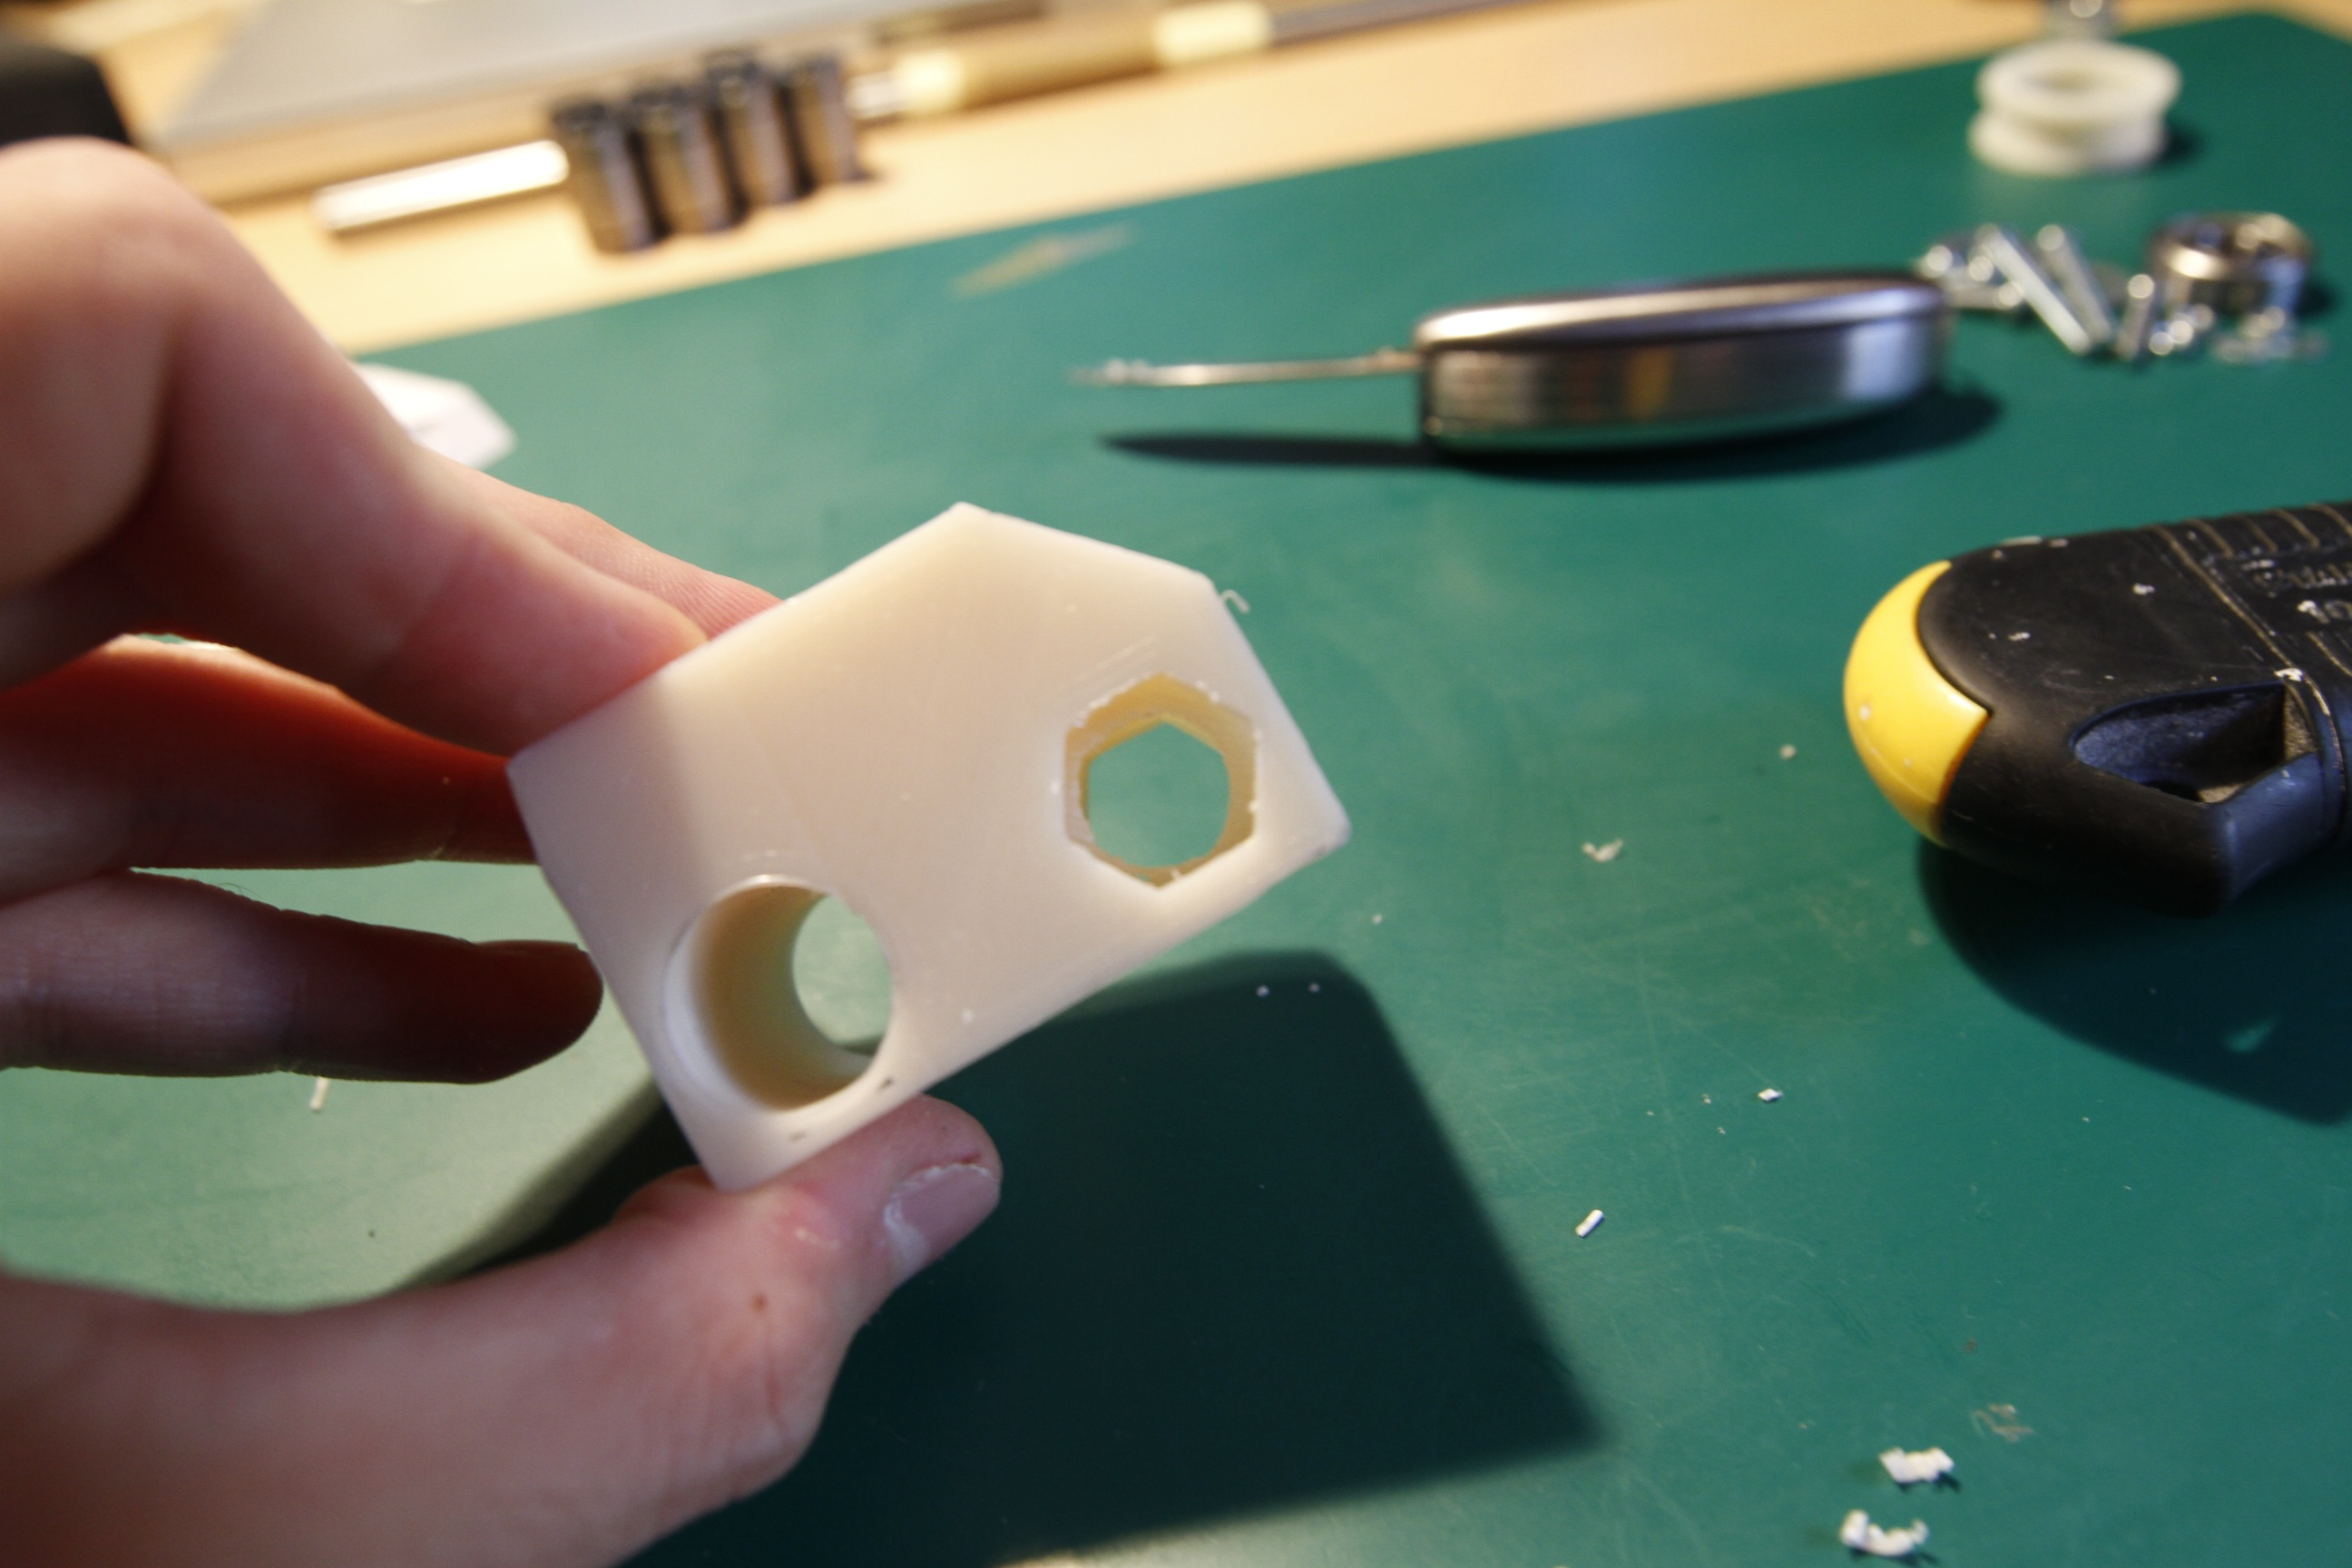
\includegraphics[width=\textwidth]{../../Fotos/49.jpg}
			                \caption{Agujero Pasante}
			                \label{fig:agujero.pasante}
			        \end{subfigure}
			        \caption{Retocando Piezas}\label{fig:agujero.xidlr}
			\end{figure}
			Una vez hecho los agujeros pasantes, será necesario empotrar las tuercas en las bases de las piezas Xmotor y X idlr como se ve en la figura ~\ref{fig:tuercas.empotradas}\\
			\begin{figure}[!htp]
				\centering
				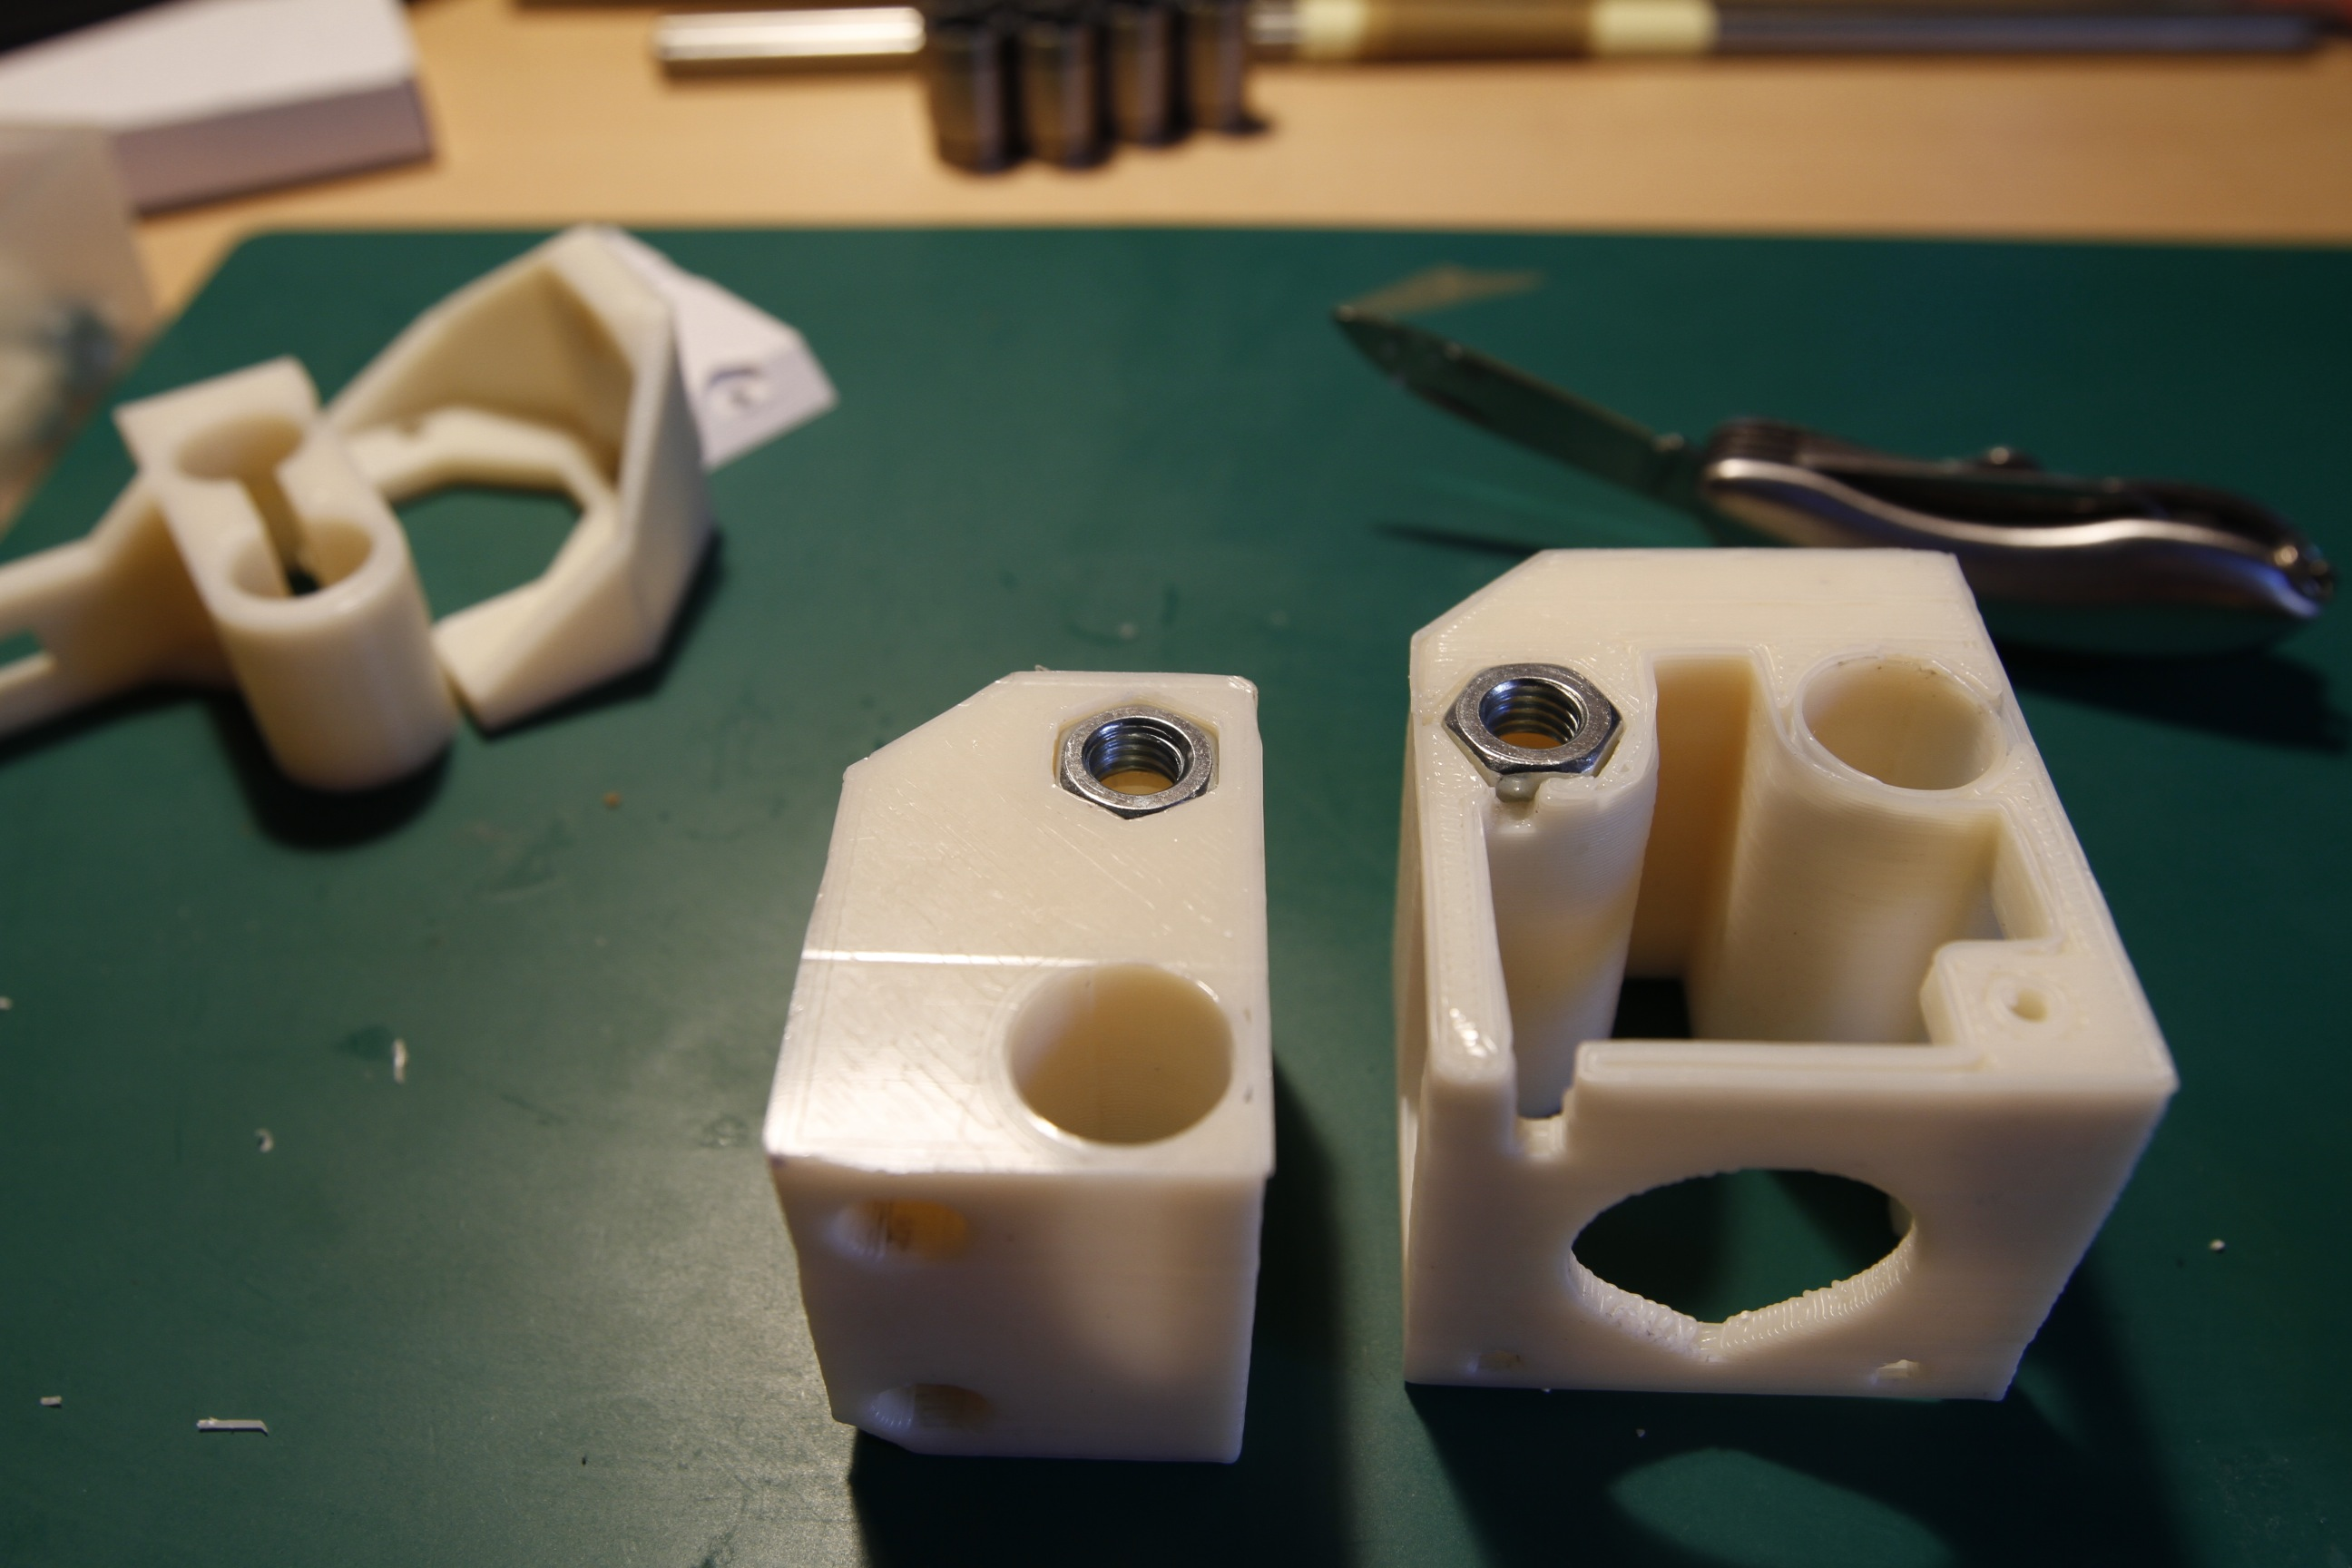
\includegraphics[width=0.6\textwidth]{../../Fotos/50.jpg}
				\caption{Tuercas empotradas}
				\label{fig:tuercas.empotradas}
			\end{figure}
			El siguiente paso es colocar el motor del eje X en la pieza X motor. Lo primero de todo será colocar la polea de 2.5 en el vástago del motor. Una vez colcoado atornillaremos el motor a la pieza.\\
			\begin{figure}[!htp]
				\centering
				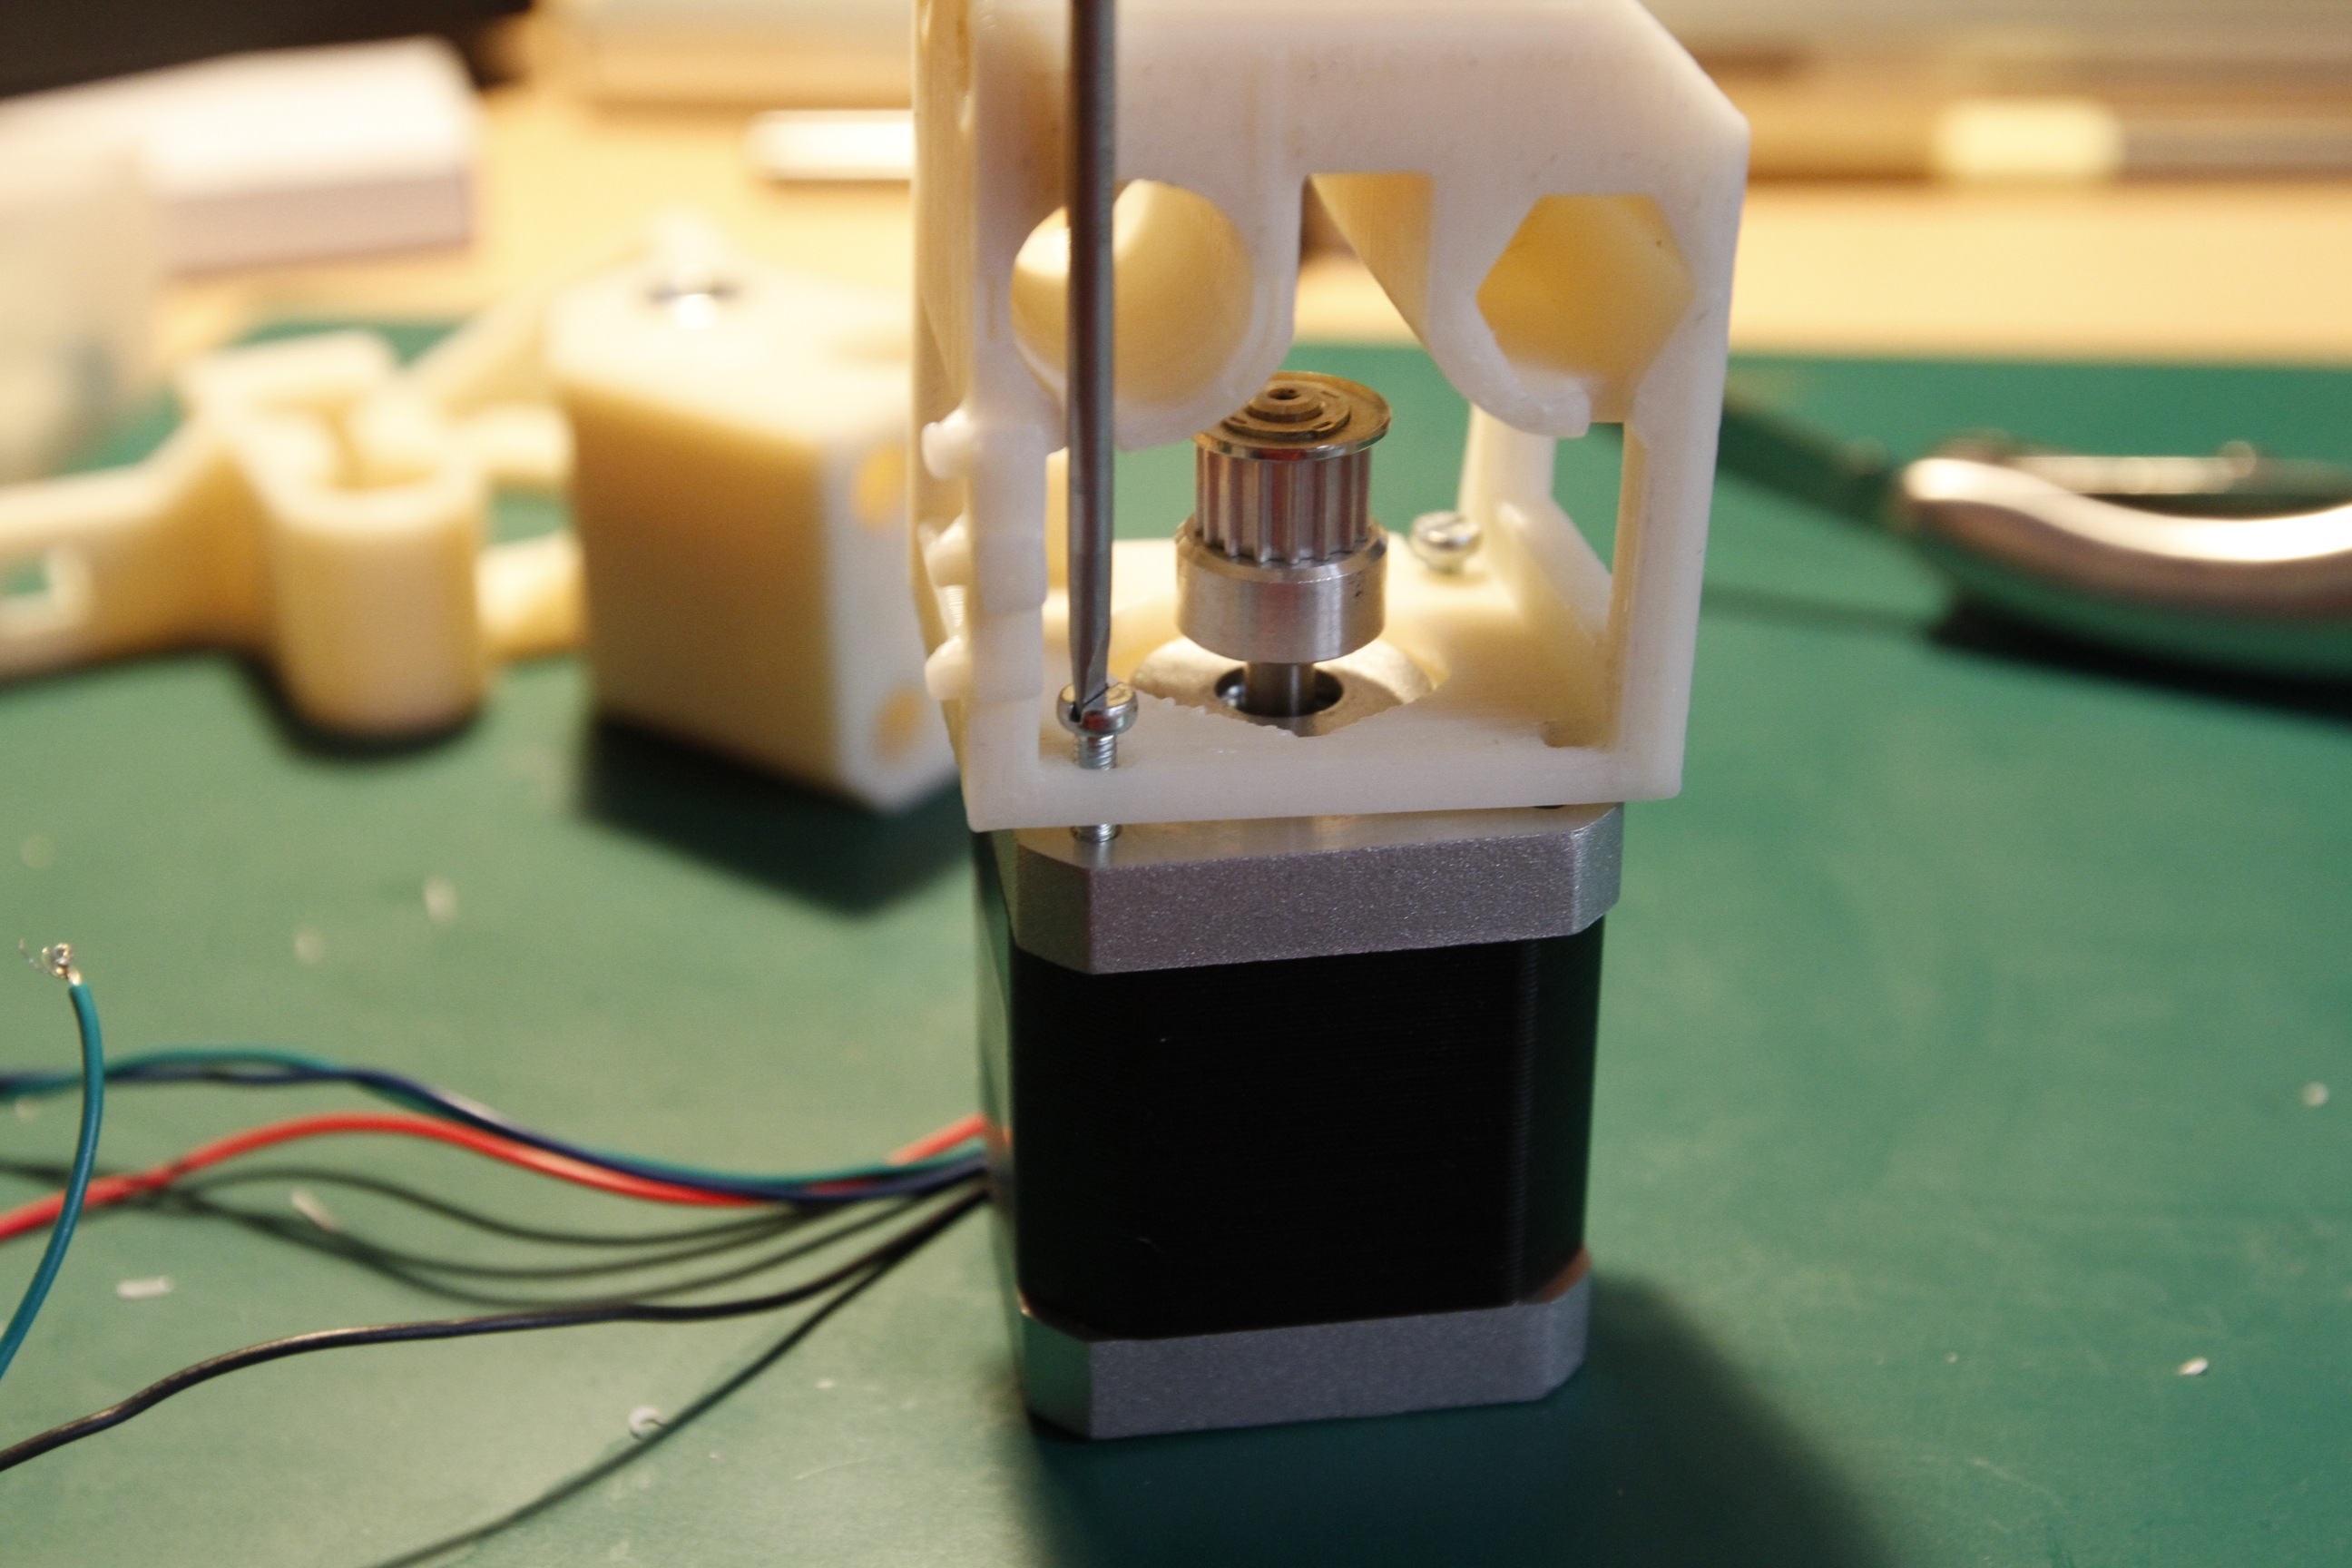
\includegraphics[width=0.6\textwidth]{../../Fotos/54.jpg}
				\caption{Atornillar motor a la pieza}
				\label{fig:motor.ejex}
			\end{figure}
			Primero atornillaremos el tornilo que está en la parte de abajo y a continuación las superiores, una vez que están los tres tonillos presentados en sus respectivos agujeros, será momento de apretarlos lo más fuerte posible.\\
			A continuación introduciremos un rodamiento lineal en las piezas Bearin guide. Para ello utilizaremos un poco de acetona para unir ambas partes al rodamiento y que quede fijo\\
			\begin{figure}[!htp]
				\centering
				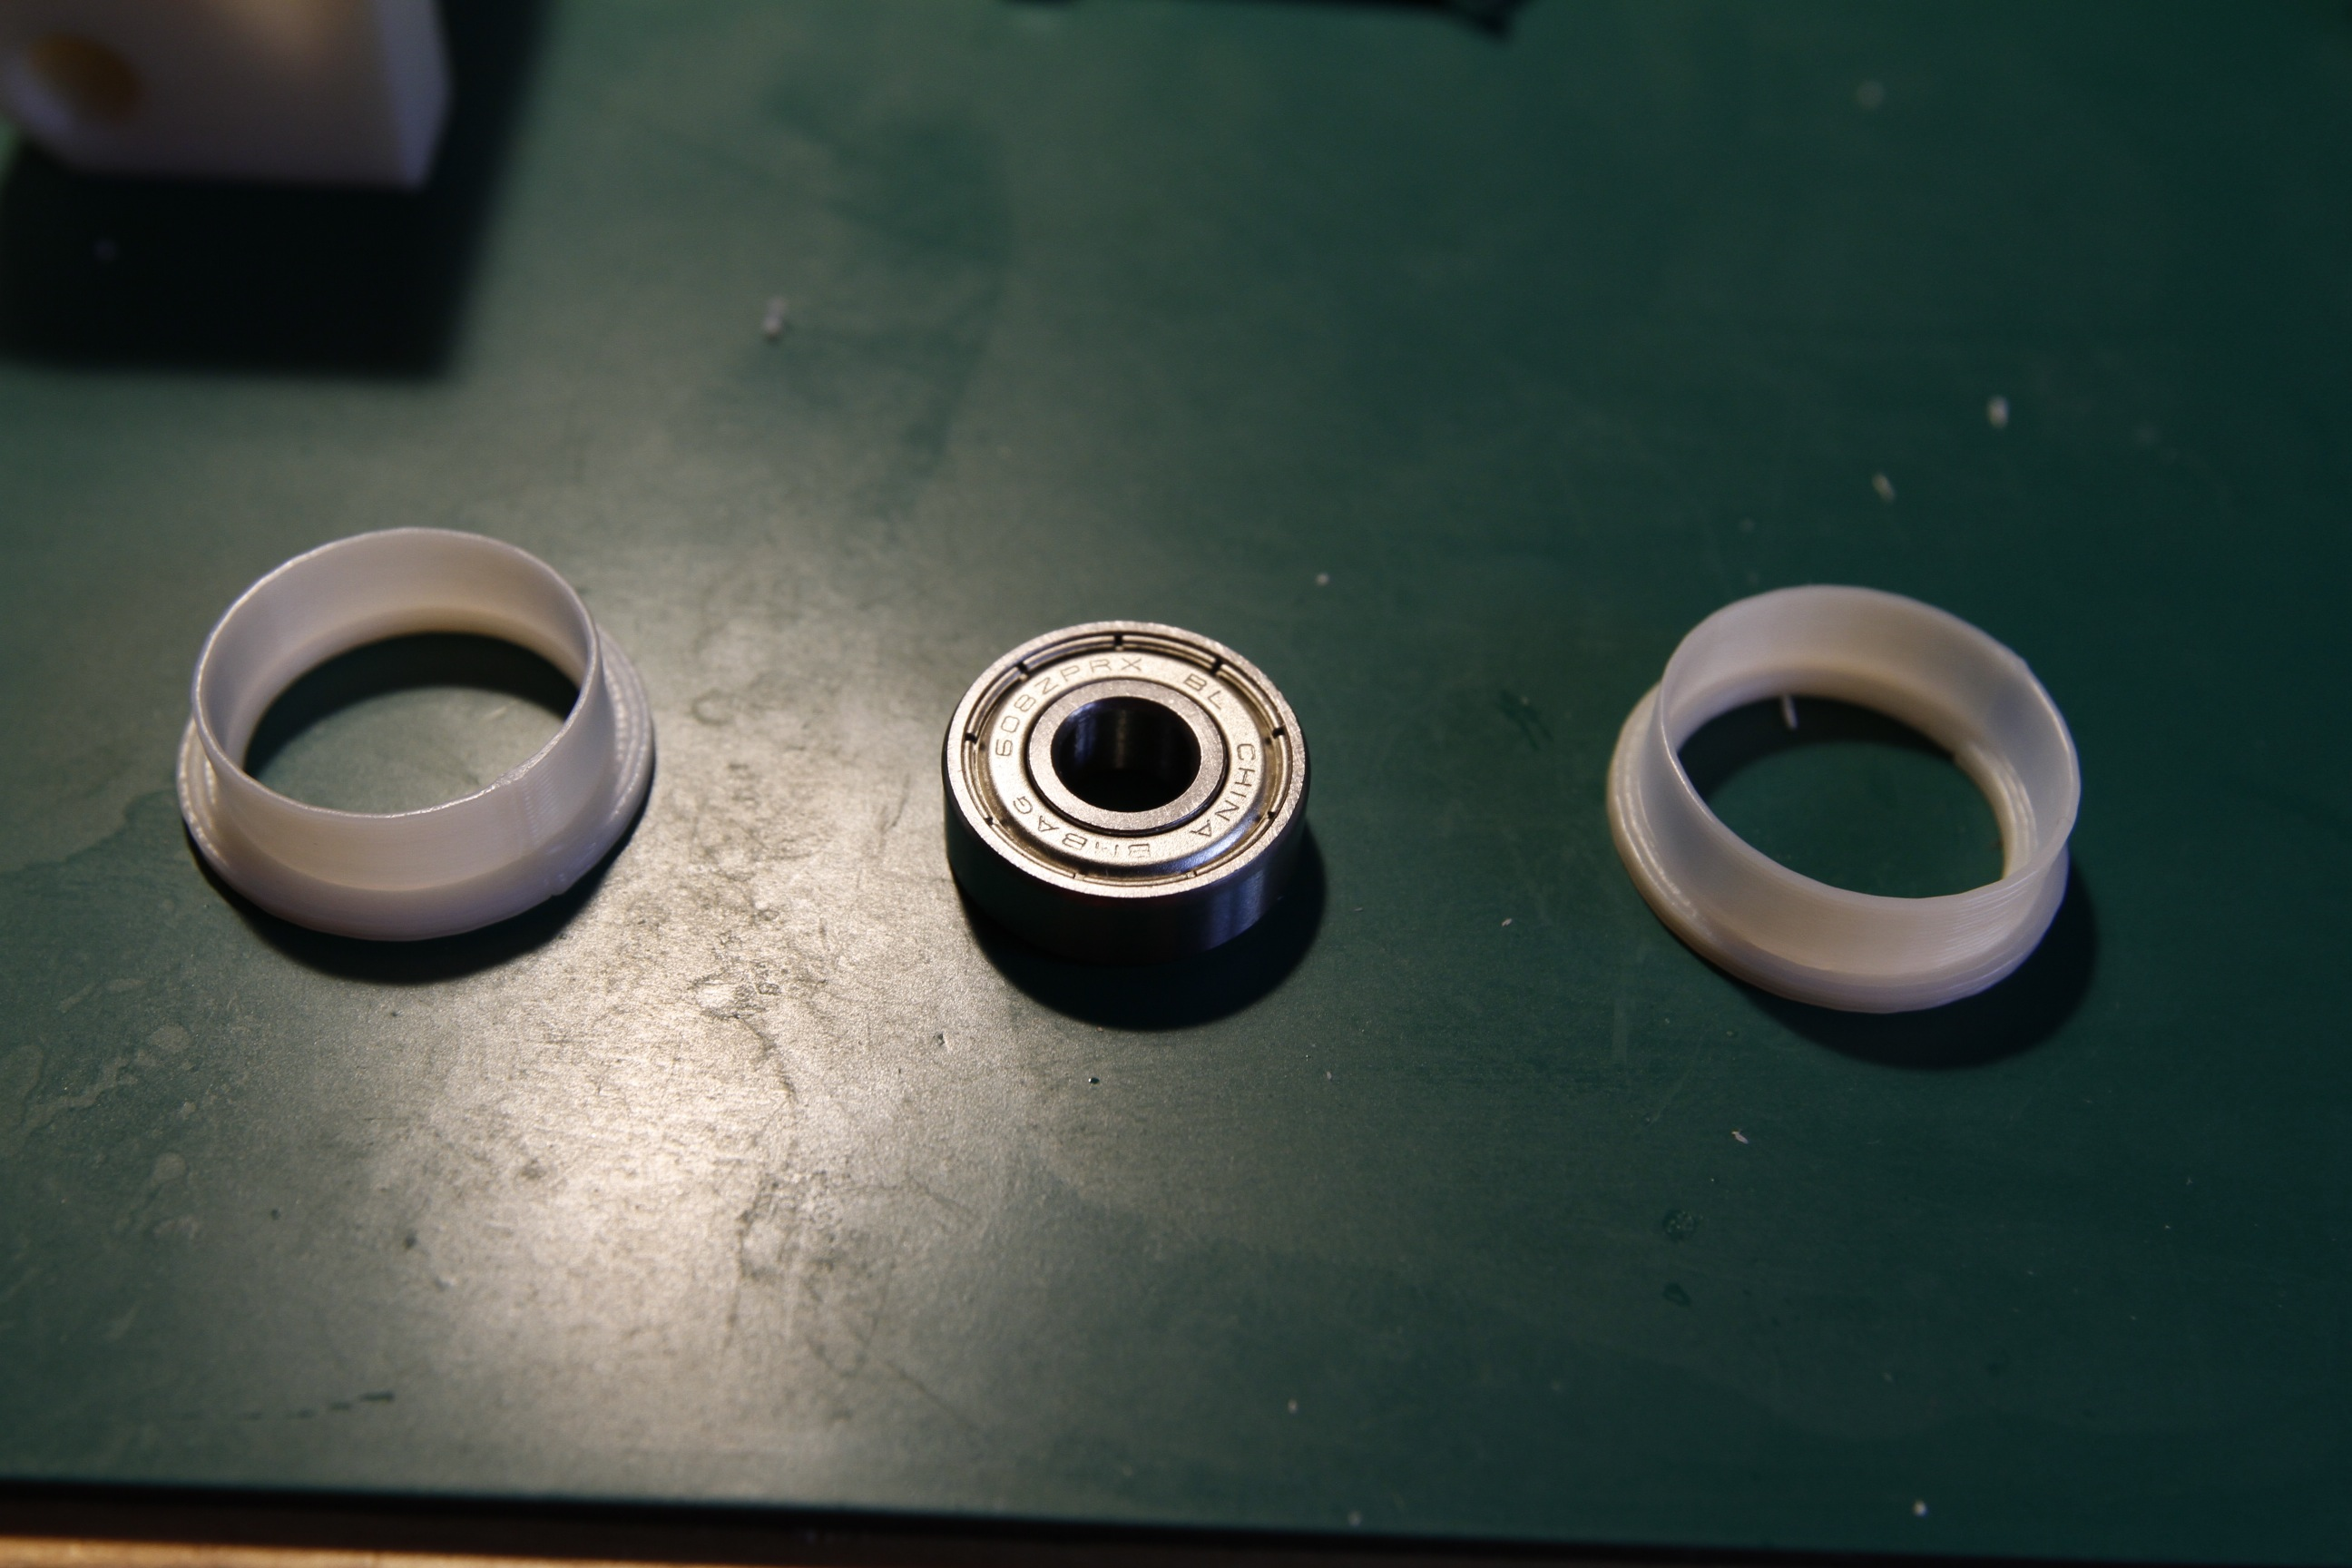
\includegraphics[width=0.6\textwidth]{../../Fotos/55.jpg}
				\caption{Rodamiento lineal eje X}
				\label{fig:rodamiento.ejex}
			\end{figure}
			Una vez secada la pieza, montamos el conjunto que podemos ver en la imagen ~\ref{fig:conjunto.ejex}, para luego introducirla en la pieza X idlr (Ver imagen ~\ref{fig:conjuntoxidlr.ejex}). Nos ayudamos de una llave inglesa para apretar todo.\\
			\begin{figure}[H]
			        \centering
			        \begin{subfigure}[htb]{0.4\textwidth}
			                \centering
			                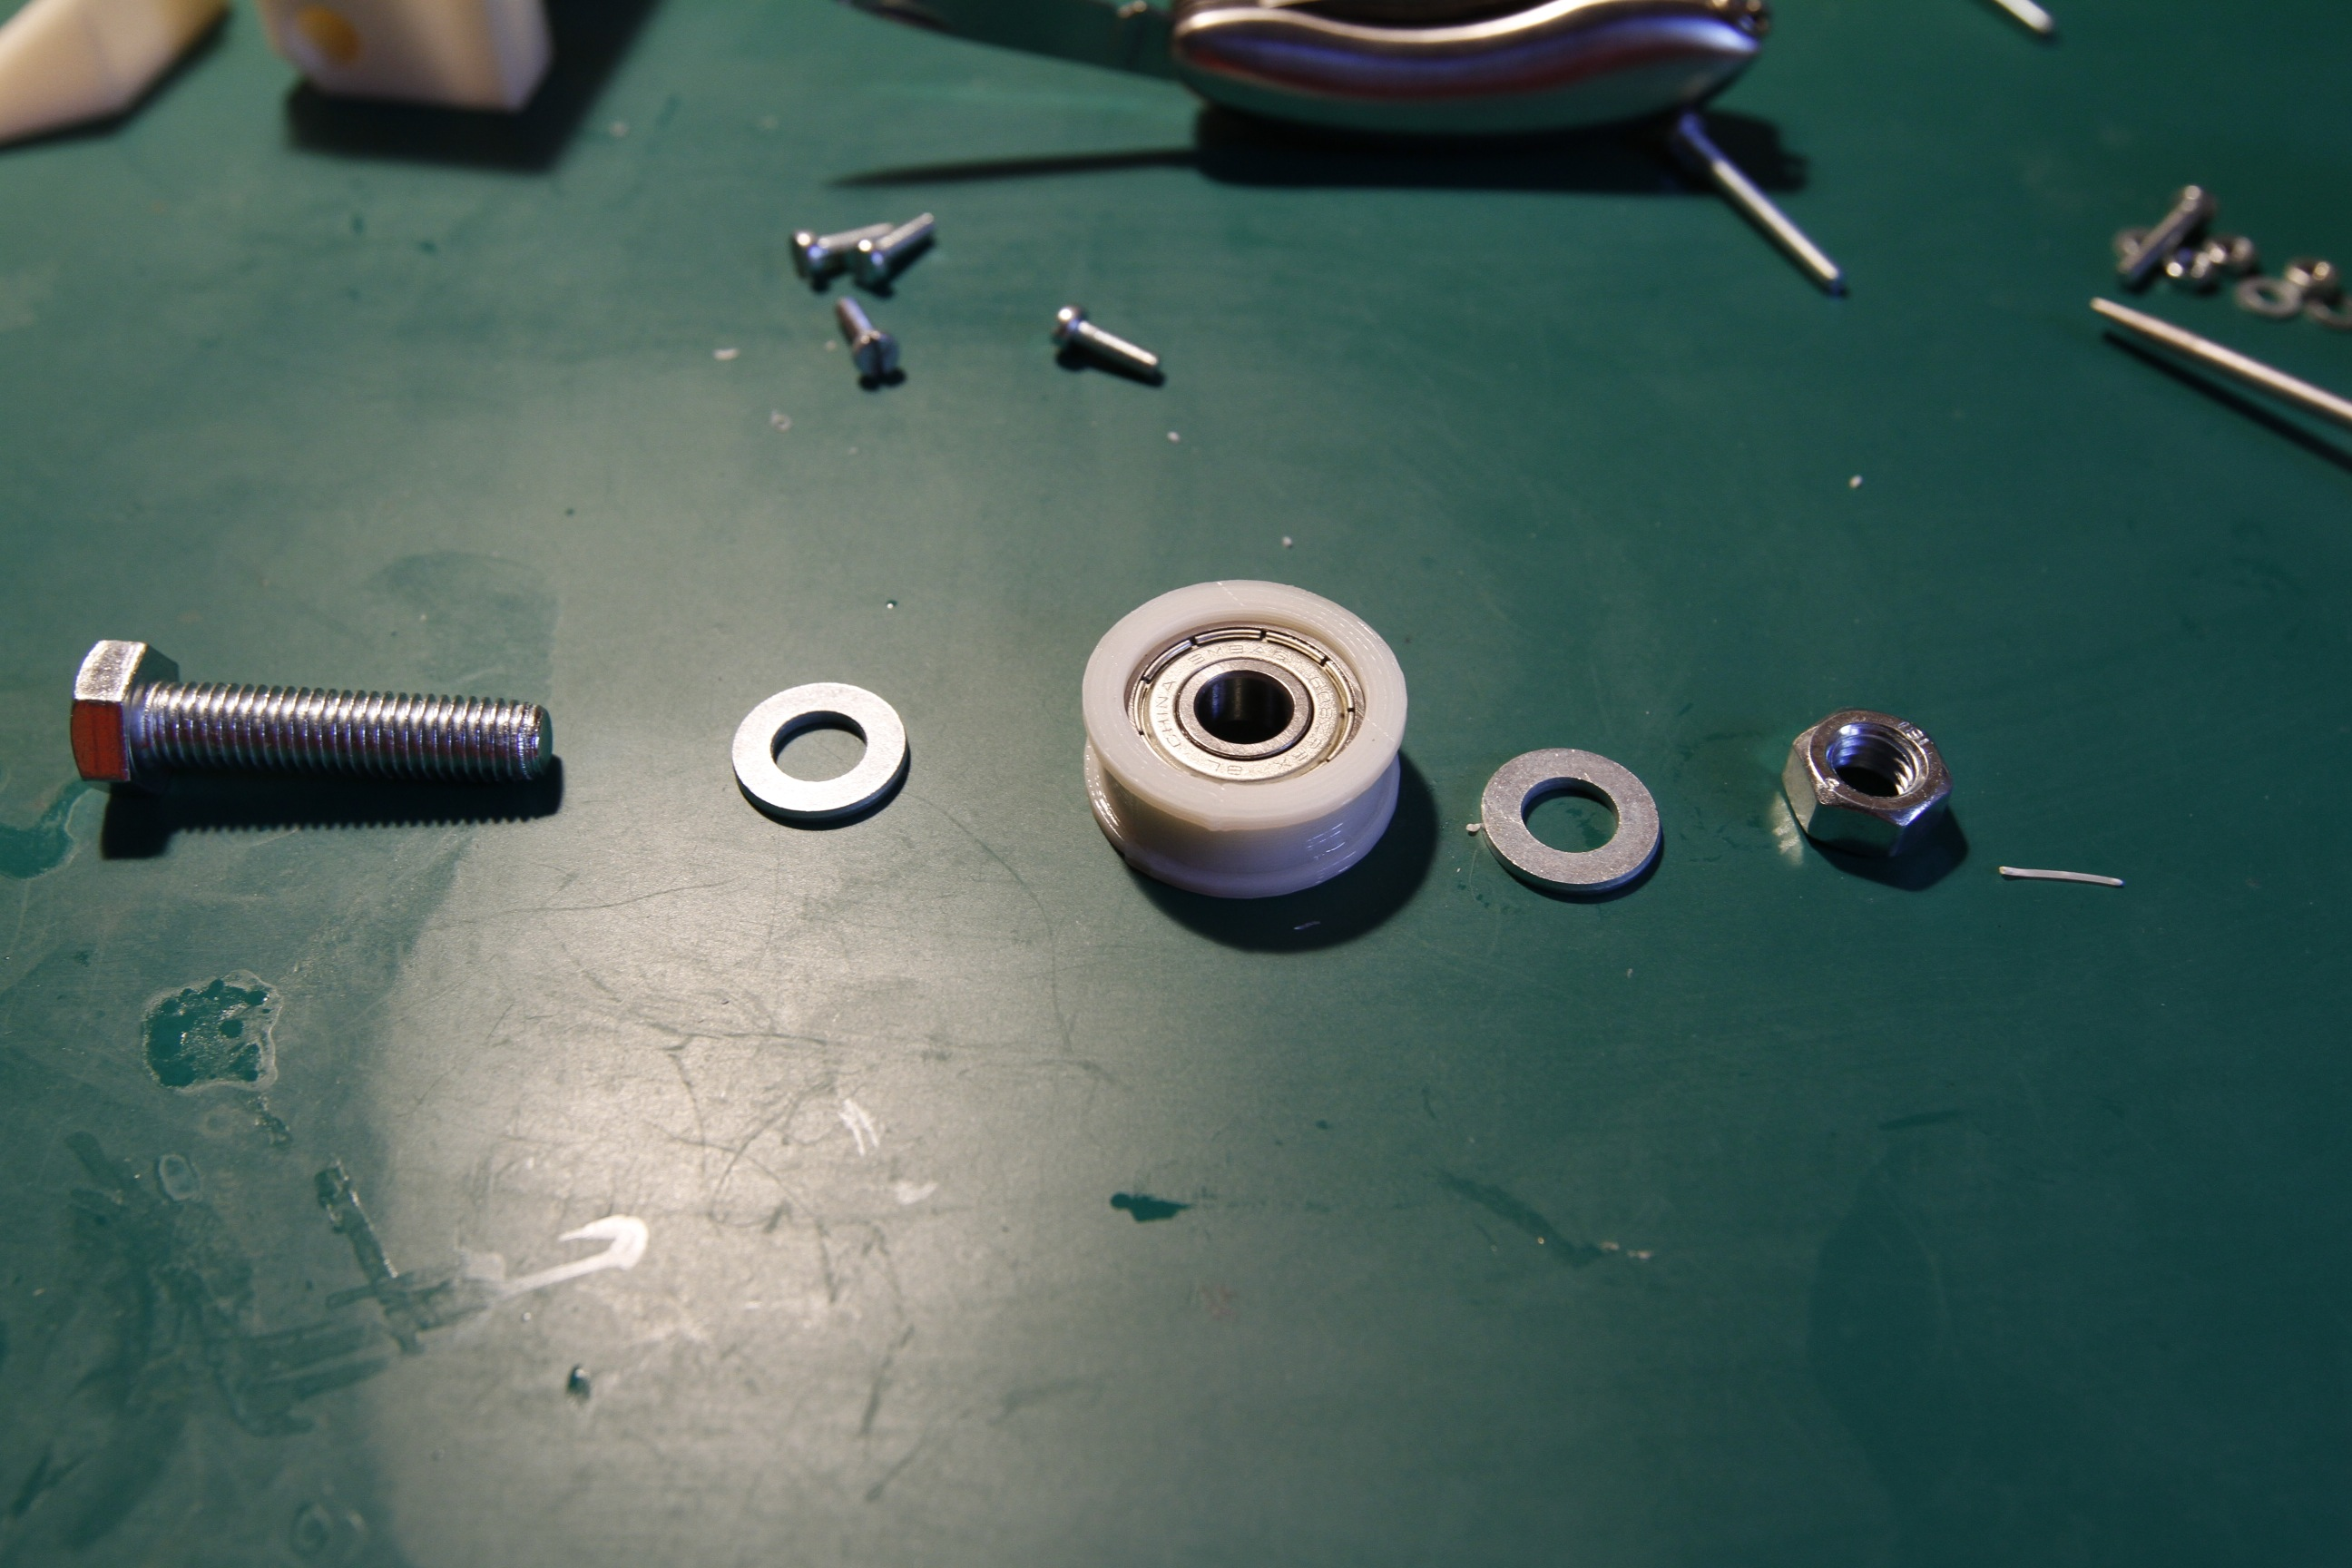
\includegraphics[width=\textwidth]{../../Fotos/56.jpg}
			                \caption{Conjunto despiezado}
			                \label{fig:conjunto.ejex}
			        \end{subfigure}
			        \begin{subfigure}[htb]{0.4\textwidth}
			                \centering
			                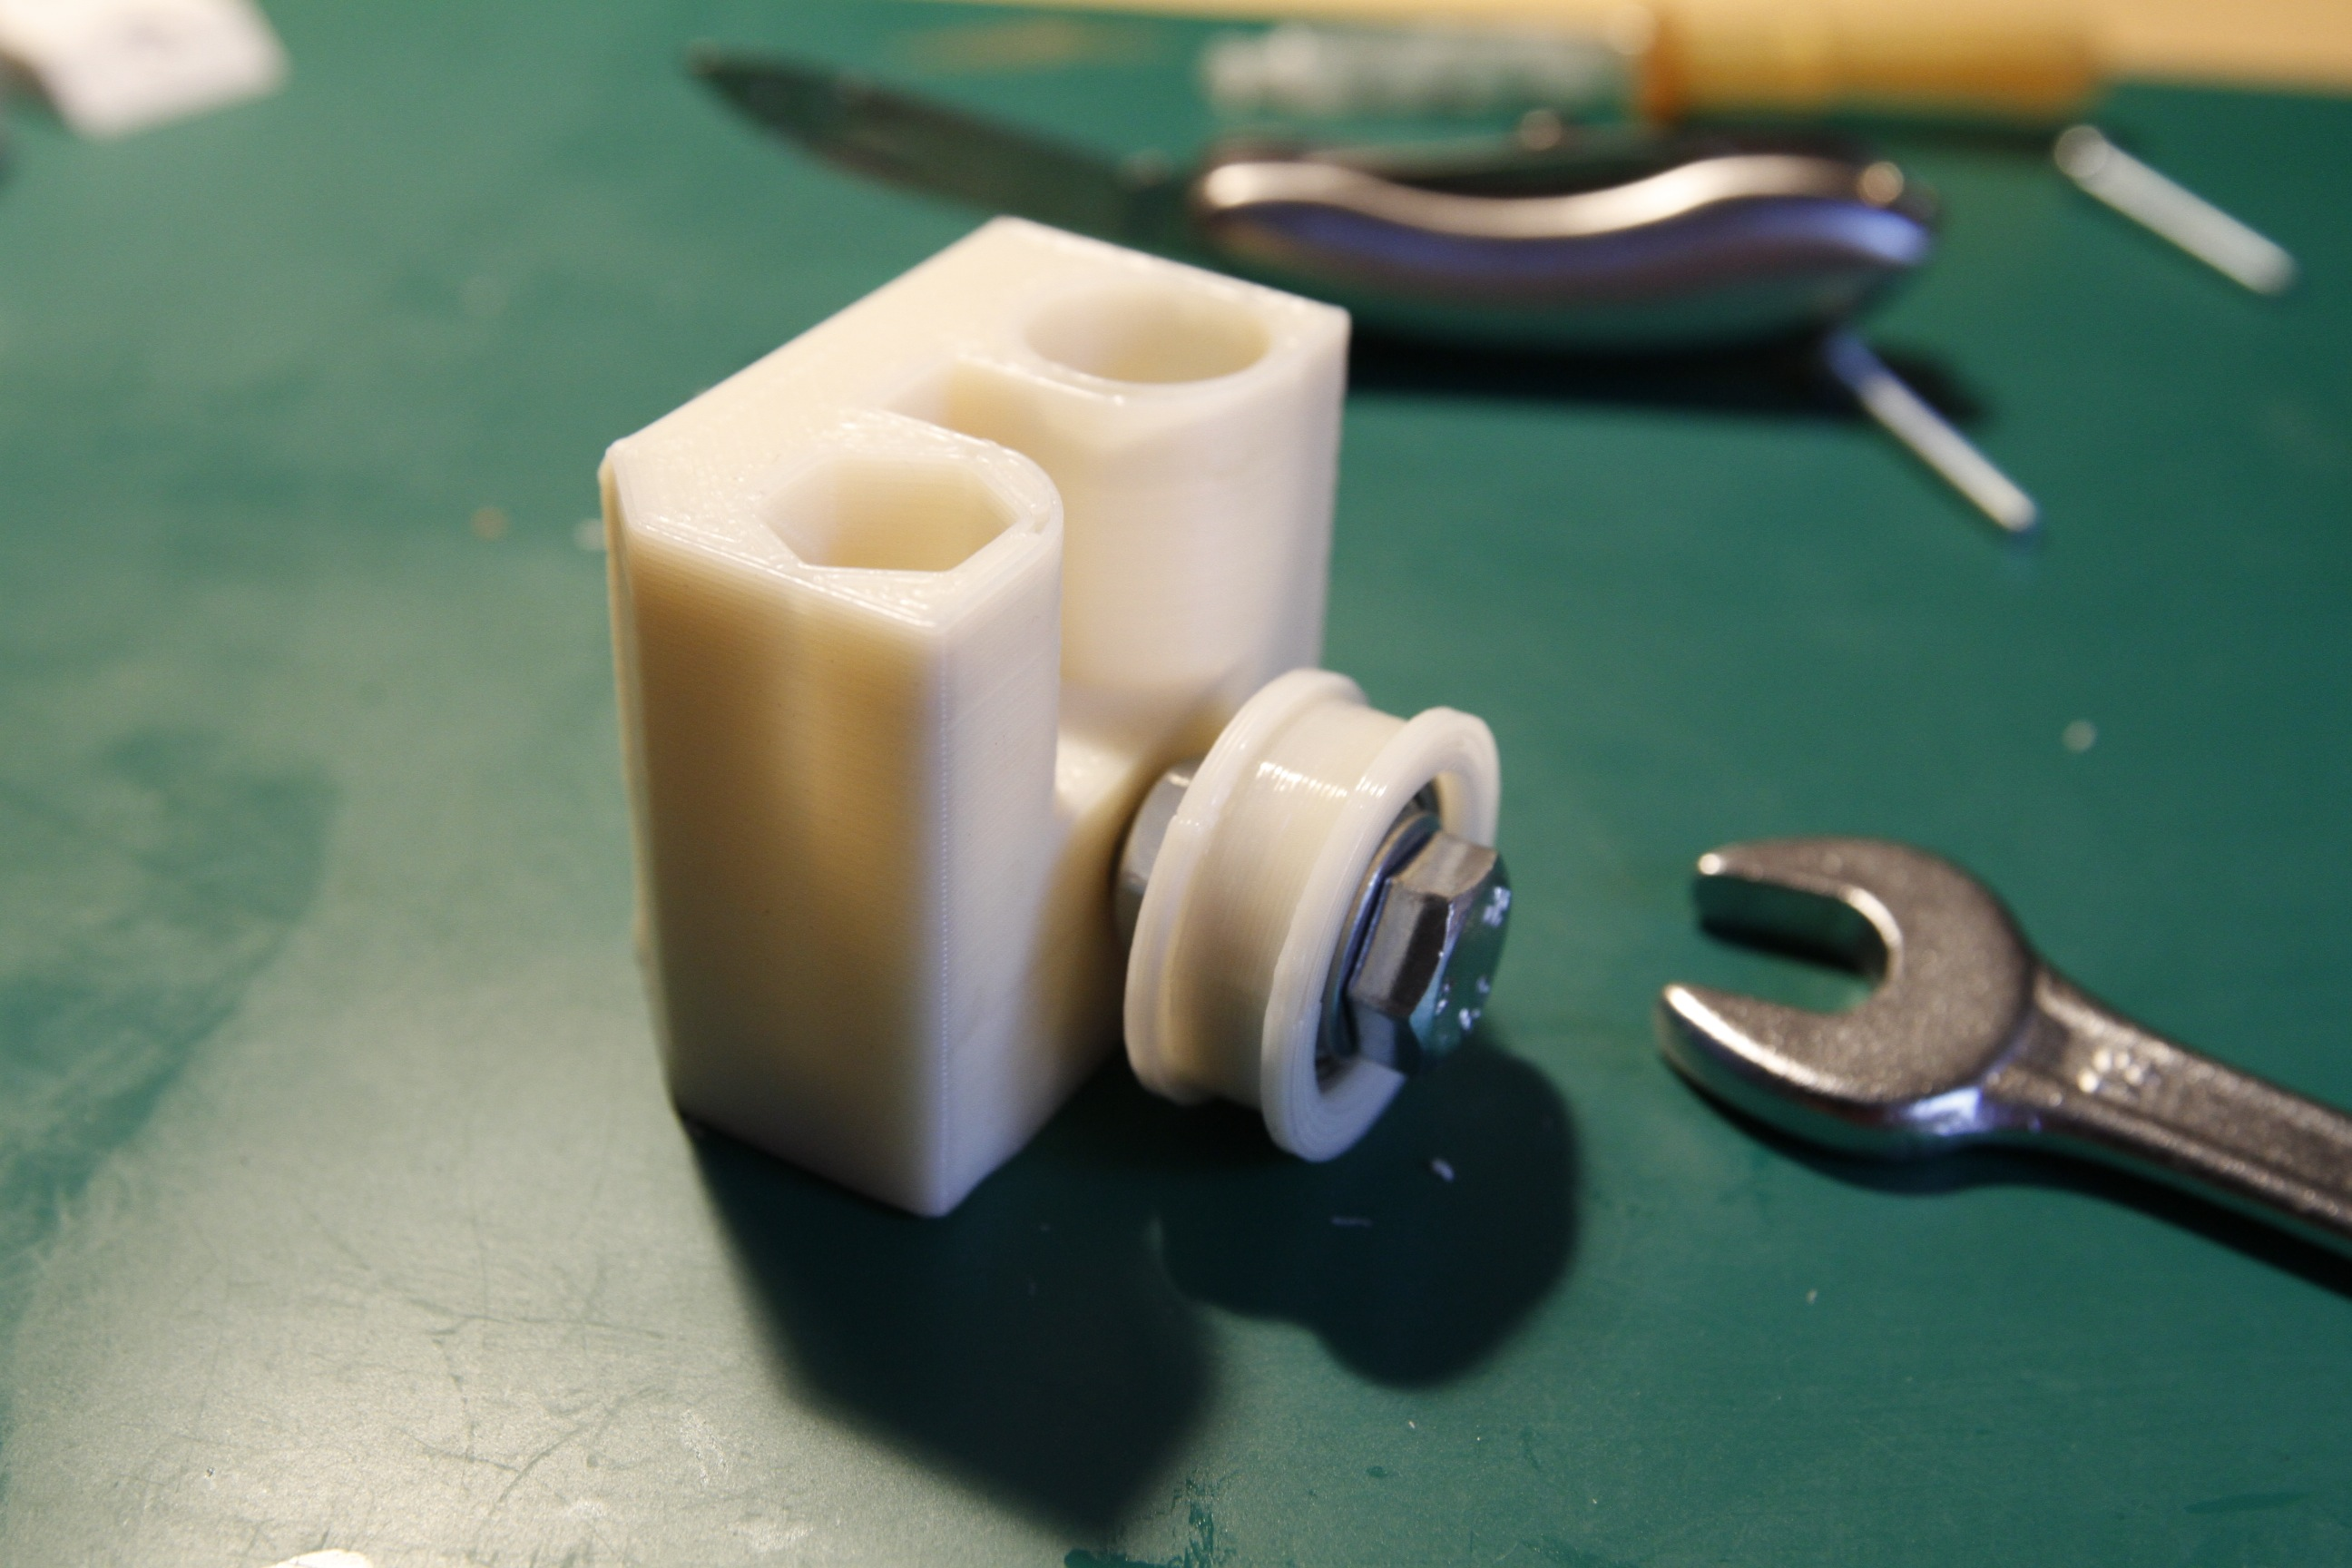
\includegraphics[width=\textwidth]{../../Fotos/57.jpg}
			                \caption{Conjunto montado}
			                \label{fig:conjuntoxidlr.ejex}
			        \end{subfigure}
			        \caption{Colocando rodamiento eje X}\label{fig:rodamientopieza.ejex}
			\end{figure}
			Pasamos ahora a montar la pieza que soporta el extrusor, en caso de que tengamos un extrusor corto, como pueda ser el J-head MkV necesitaremos añadir a la pieza X Extruder mount la pieza de adaptación, primero introduciremos los tornillos de M3x35 y M3x10 para unir ambas piezas como se ve en la figura ~\ref{fig:extrudermount.ejex}
			\begin{figure}[H]
			        \centering
			        \begin{subfigure}[htb]{0.4\textwidth}
			                \centering
							
			                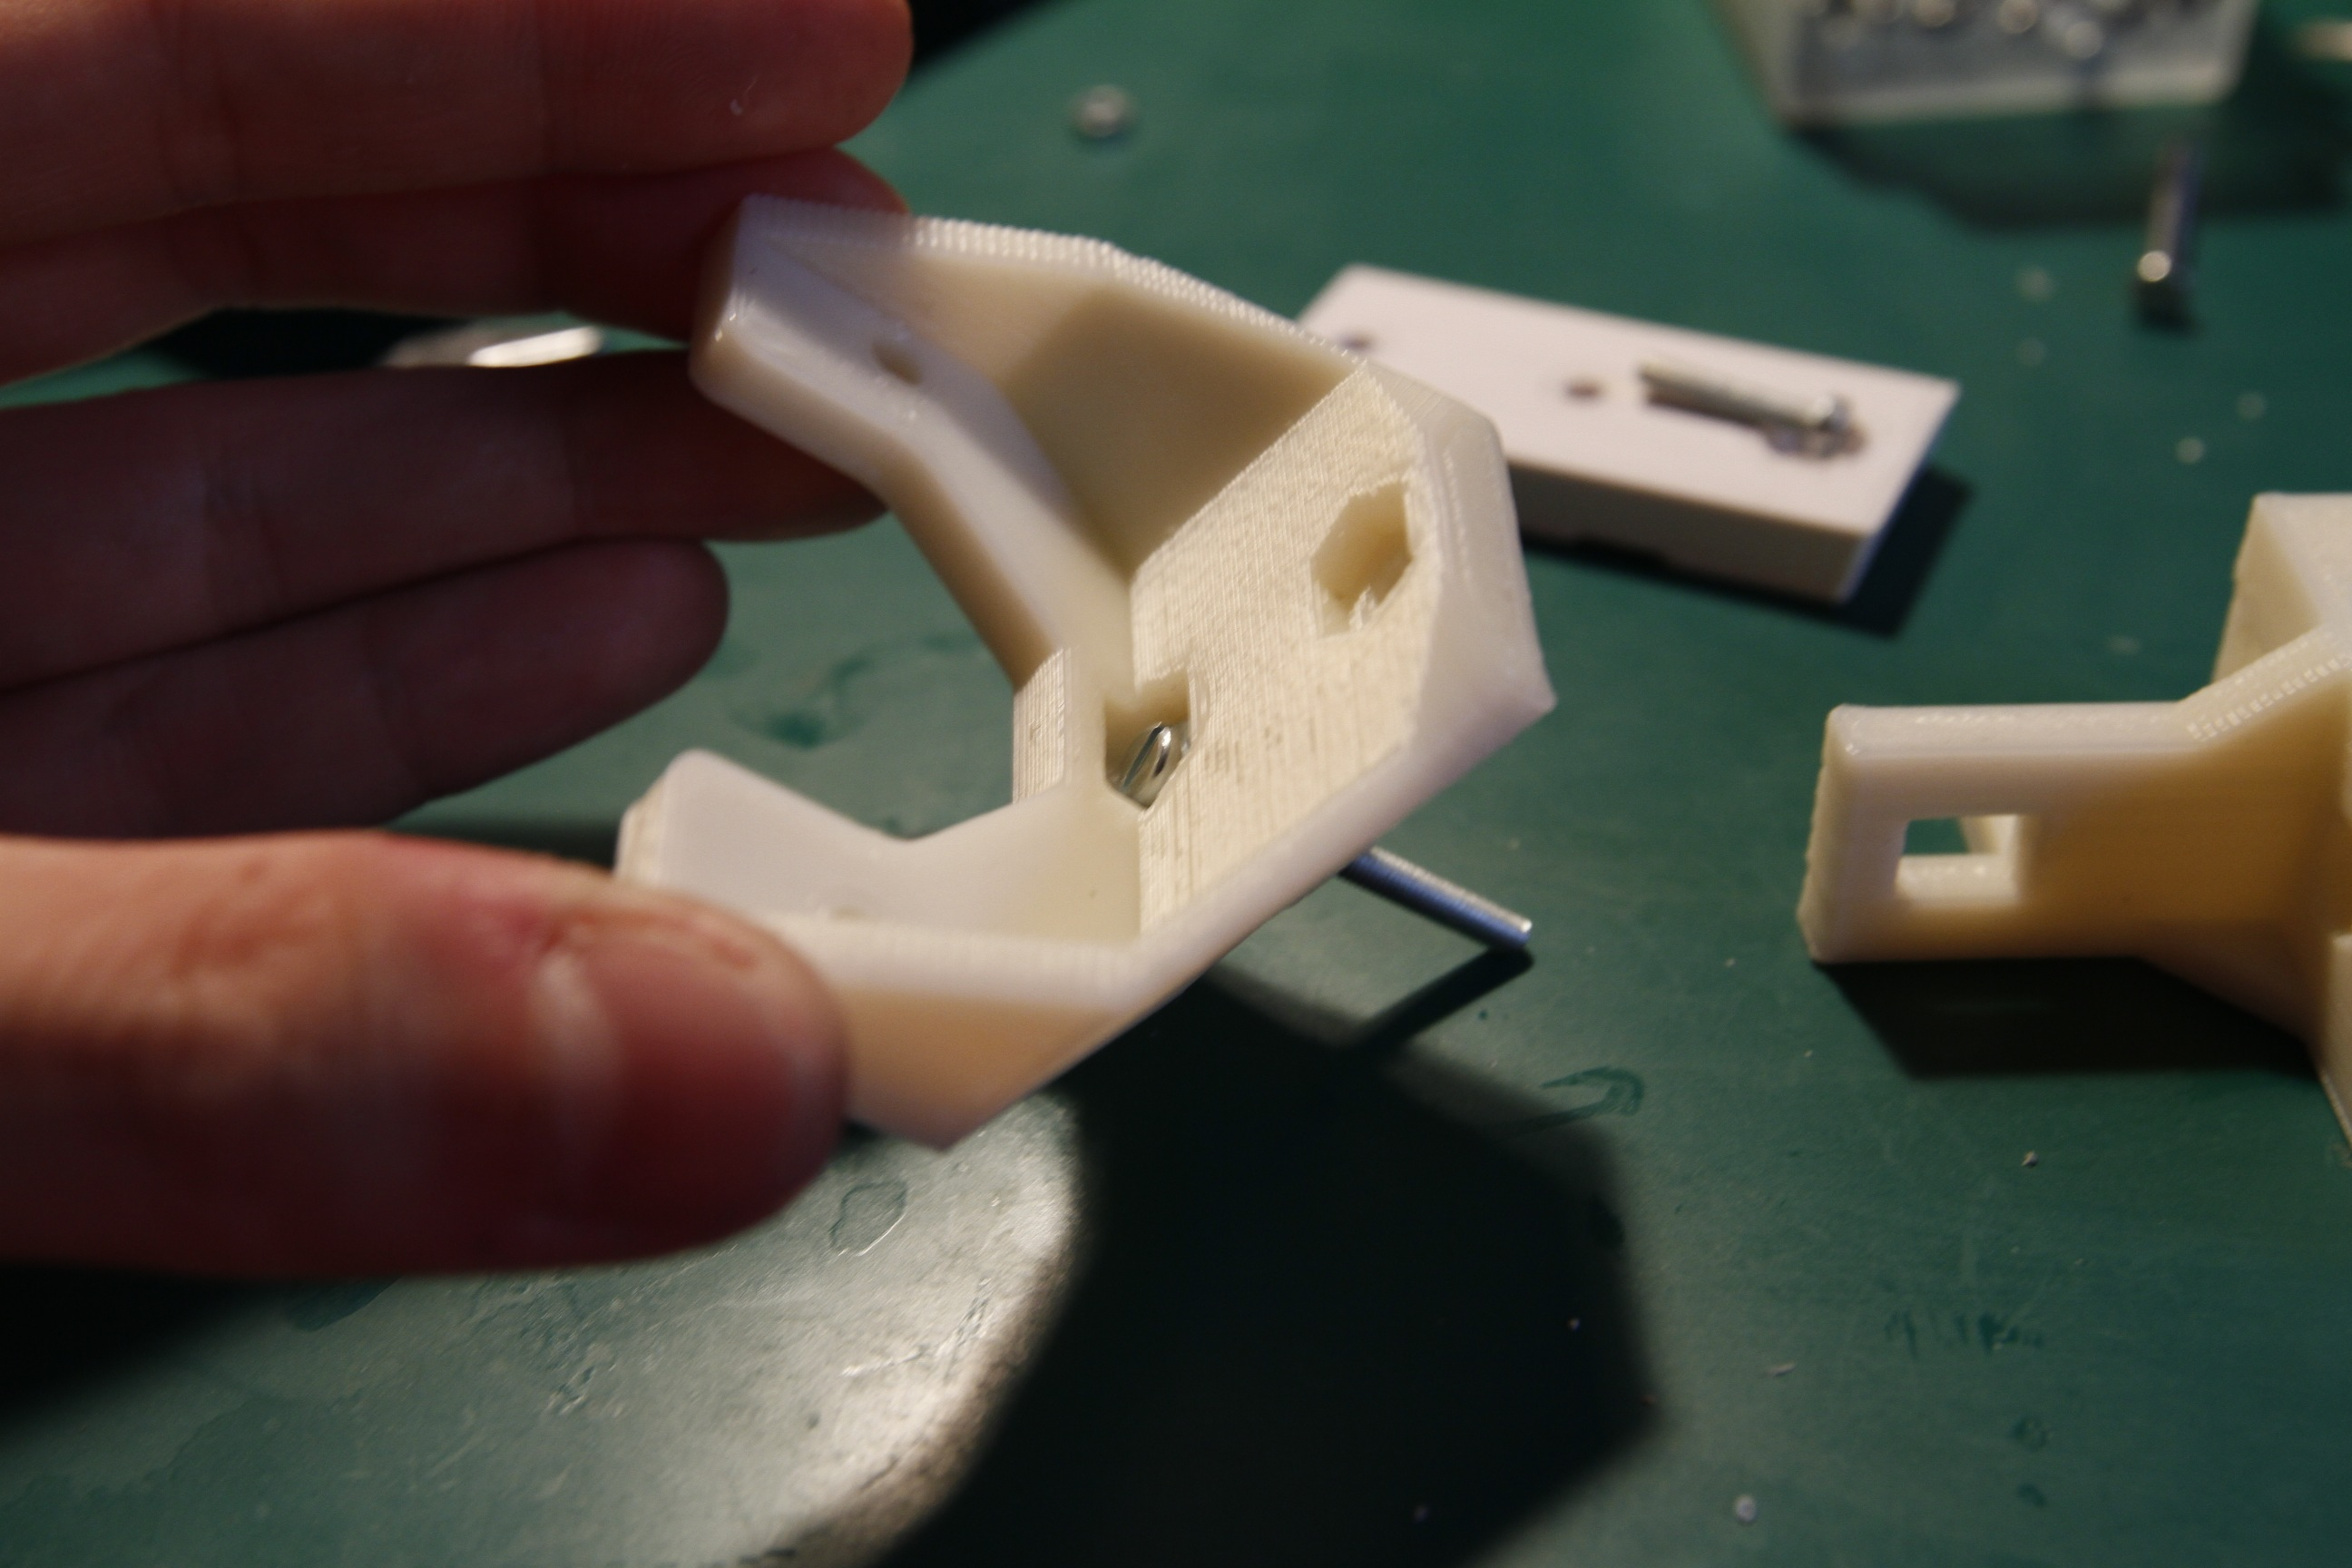
\includegraphics[width=\textwidth]{../../Fotos/58.jpg}
			                \caption{Tornillos en pieza Extruder mount}
			                \label{fig:extruder.ejex}
			        \end{subfigure}
			        \begin{subfigure}[htb]{0.4\textwidth}
			                \centering
							
			                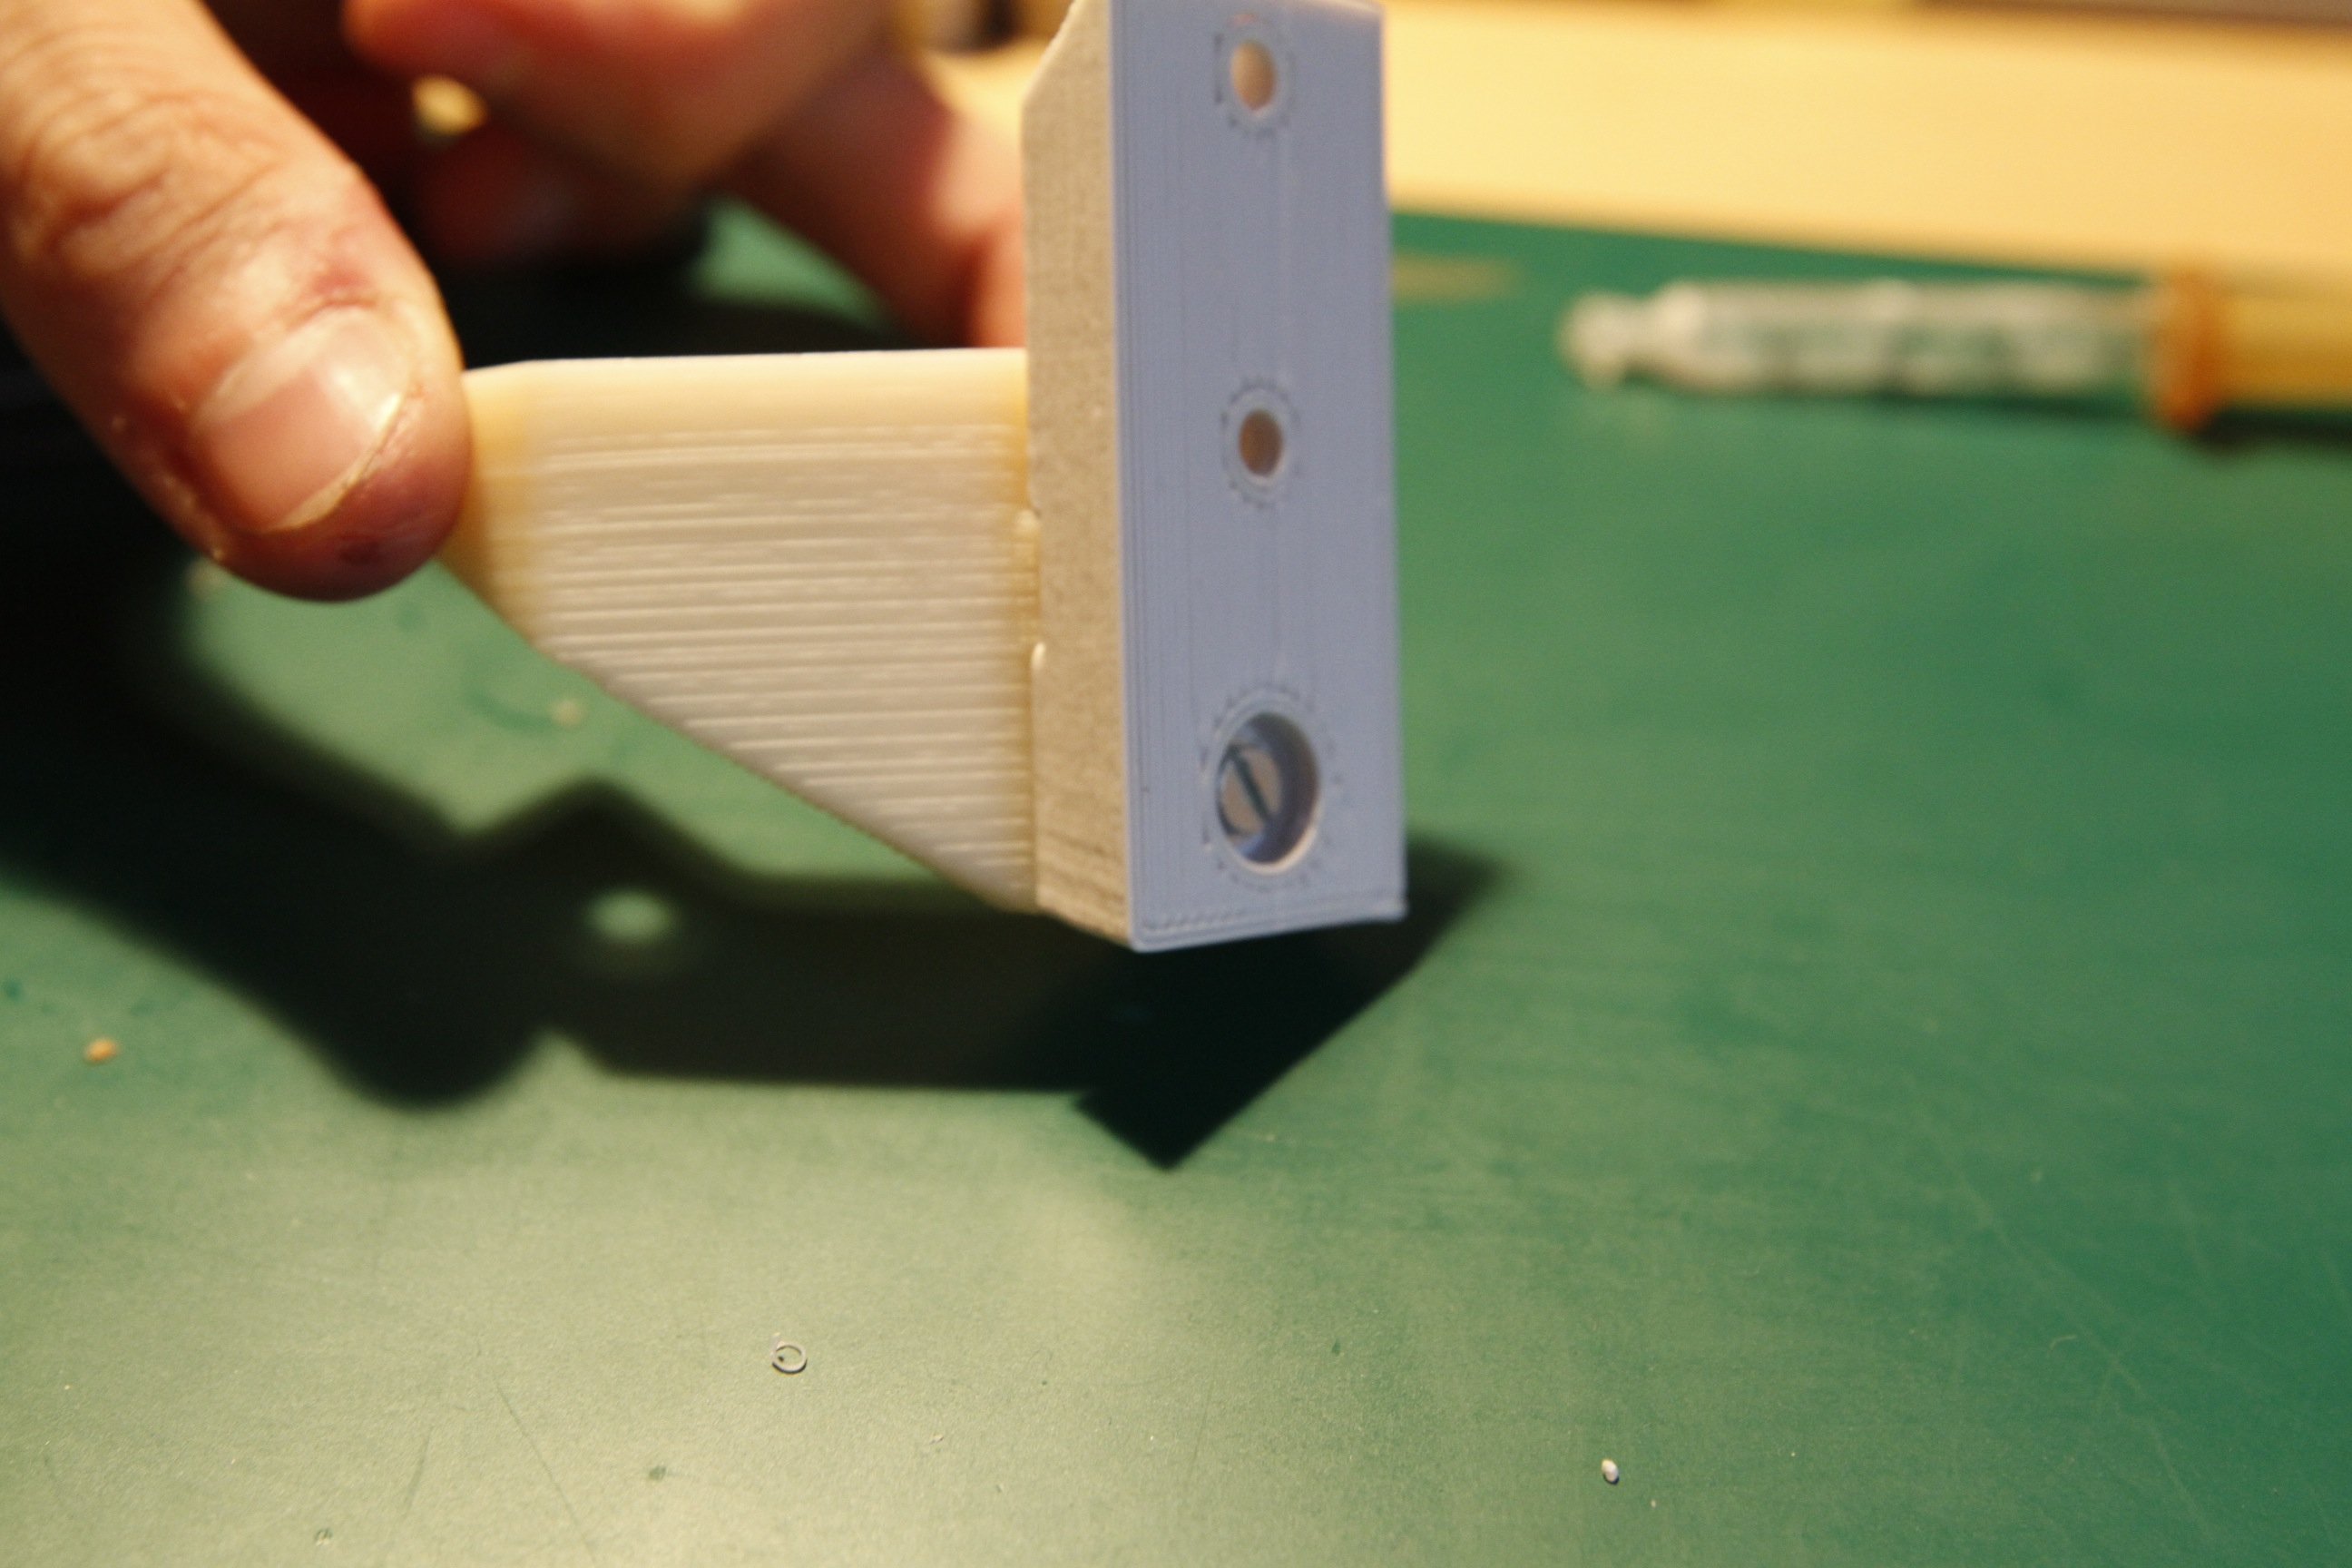
\includegraphics[width=\textwidth]{../../Fotos/59.jpg}
			                \caption{Adaptador hotend pequeño}
			                \label{fig:adaptador.ejex}
			        \end{subfigure}
			        \caption{Colocando Extruder mount del eje X}\label{fig:extrudermount.ejex}
			\end{figure}
			Para terminar, unimos la pieza X carriege con un tornillo de M3x25 para tener el conjunto mostrado en la siguiente imagen:
			\begin{figure}[!htp]
				\centering
				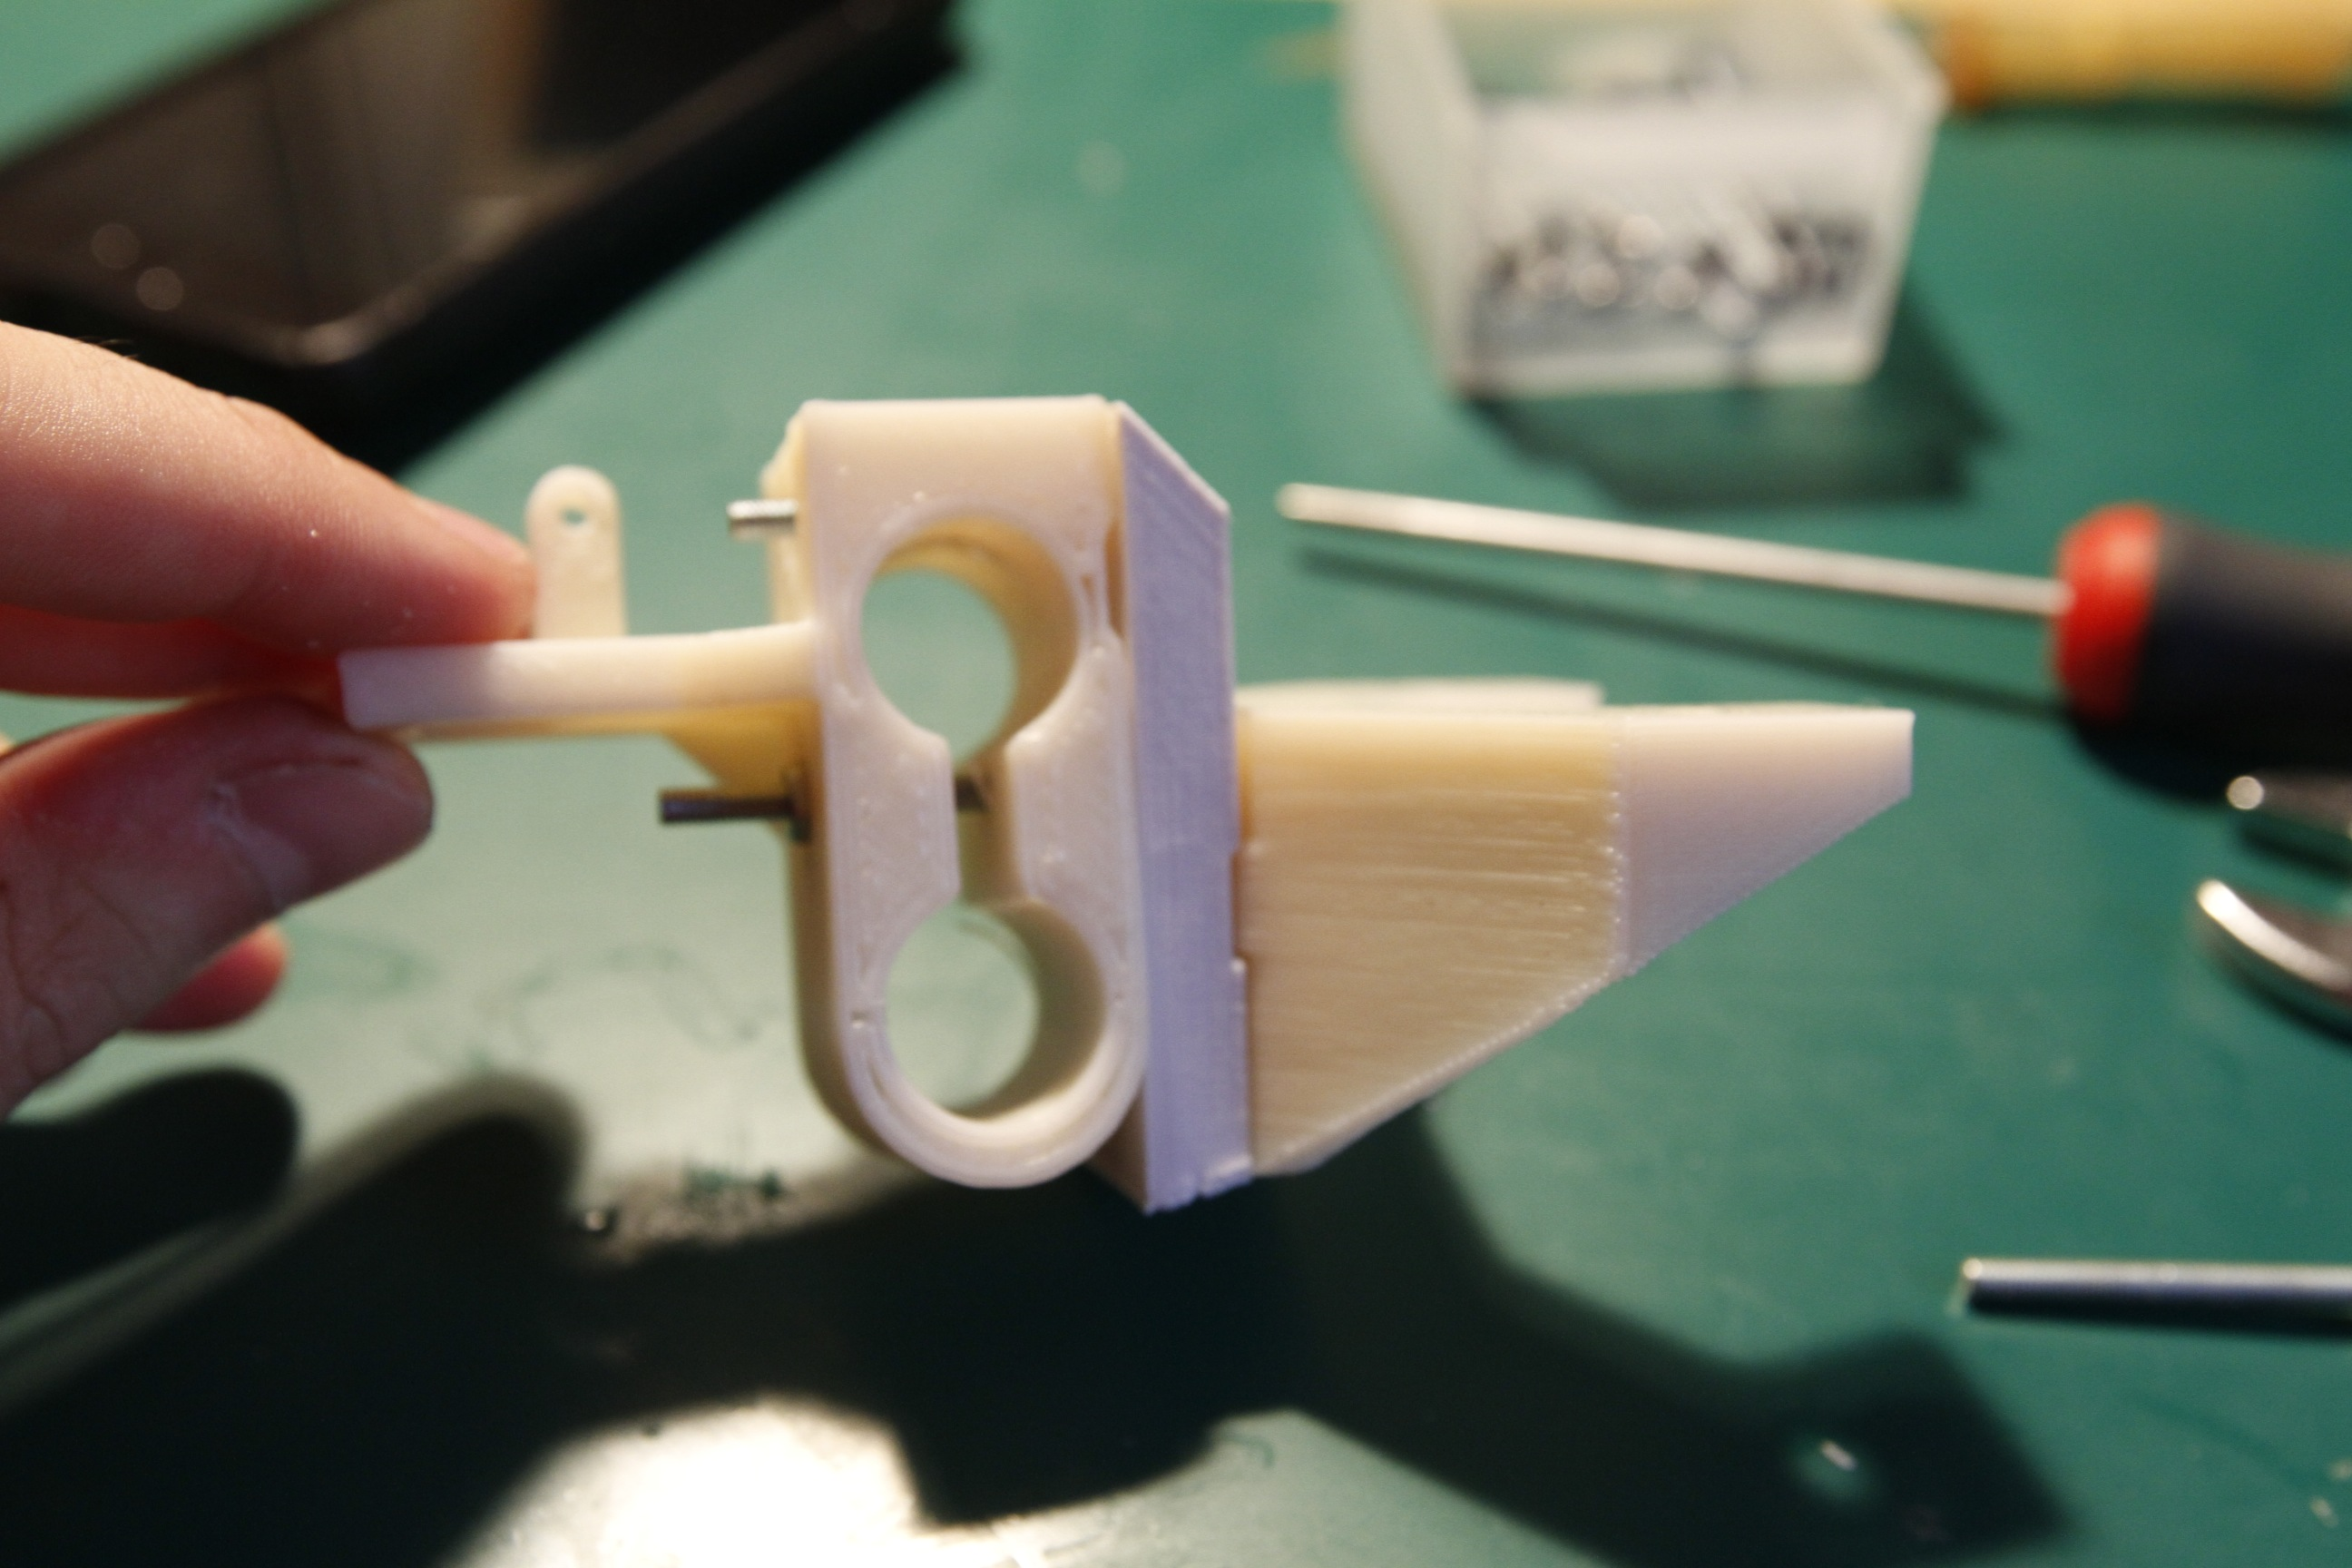
\includegraphics[width=0.6\textwidth]{../../Fotos/60.jpg}
				\caption{Conjunto Extrusor}
				%\label{fig:motor.ejex}
			\end{figure}
			Uniremos los tres conjuntos que hemos montado con las barras lisas y ya tendremos la estructura del eje X
			\begin{figure}[!htp]
				\centering
				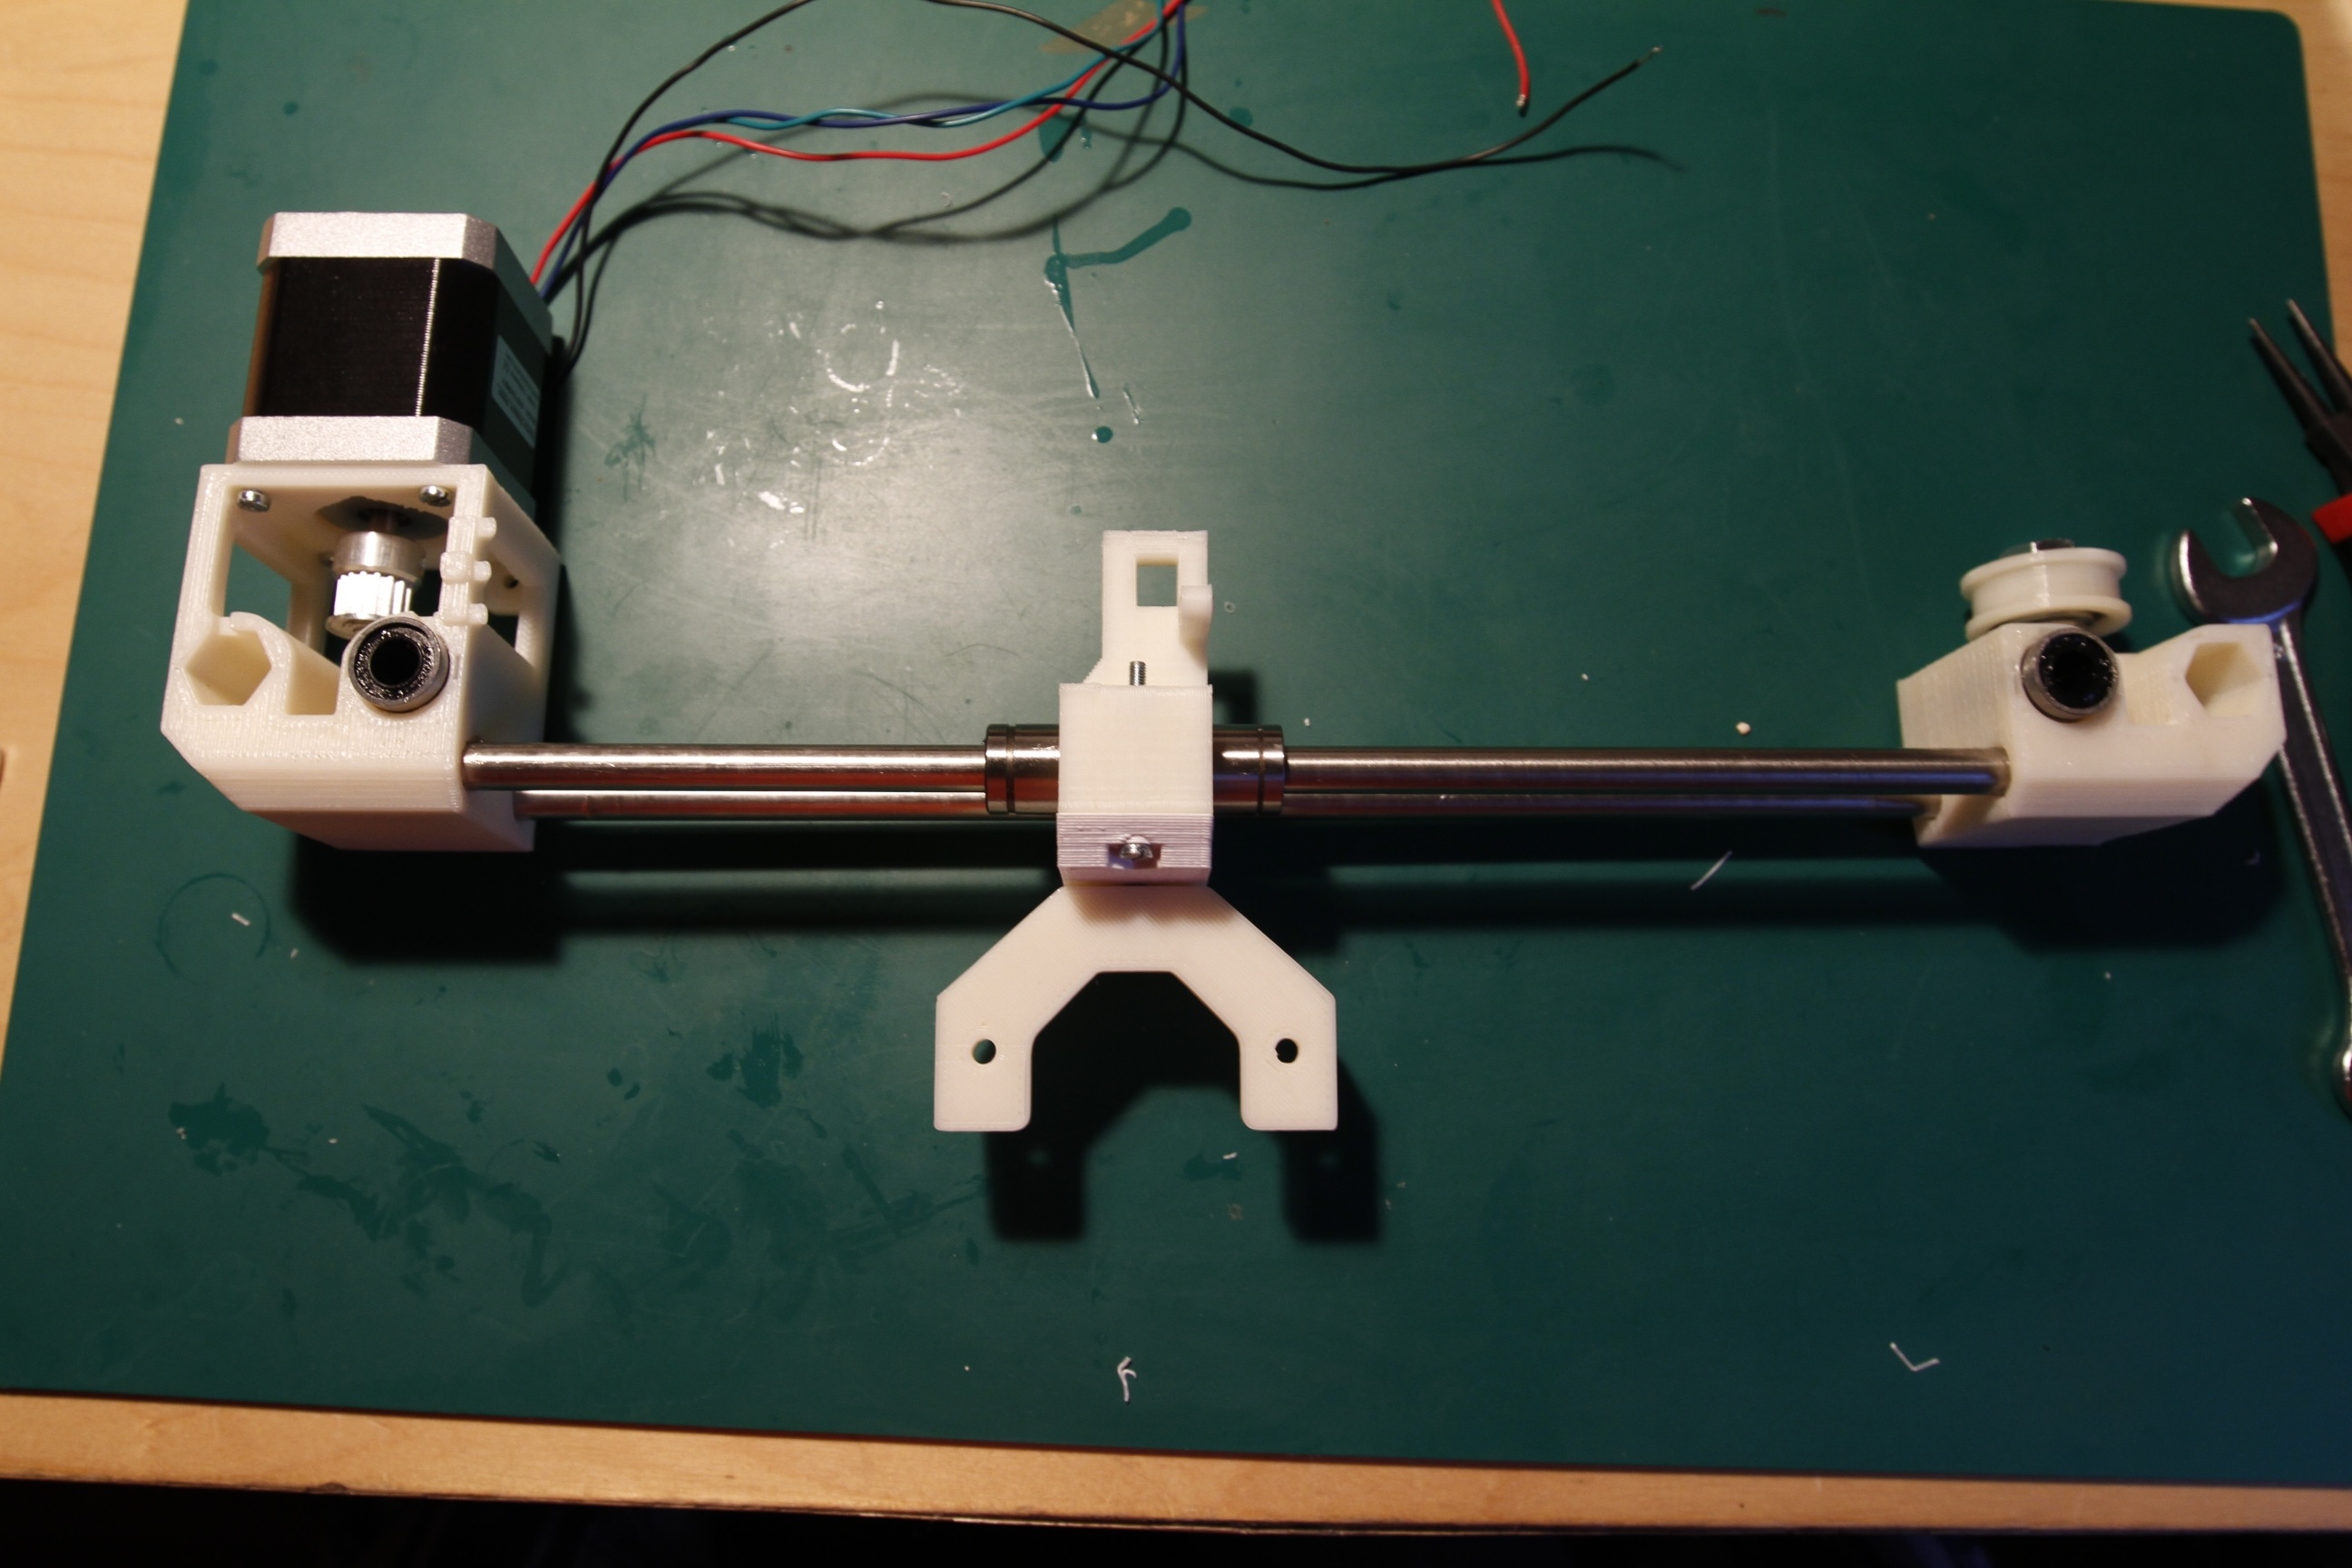
\includegraphics[width=0.6\textwidth]{../../Fotos/64.jpg}
				\caption{Eje X montado}
				%\label{fig:motor.ejex}
			\end{figure}
			A continuación, instalaremos la correa uniendo las tres piezas entre sí.Nos ayudaremos de una brida para ejercer la presión necesaria para que no se suelte nada.
			\begin{figure}[!htp]
				\centering
				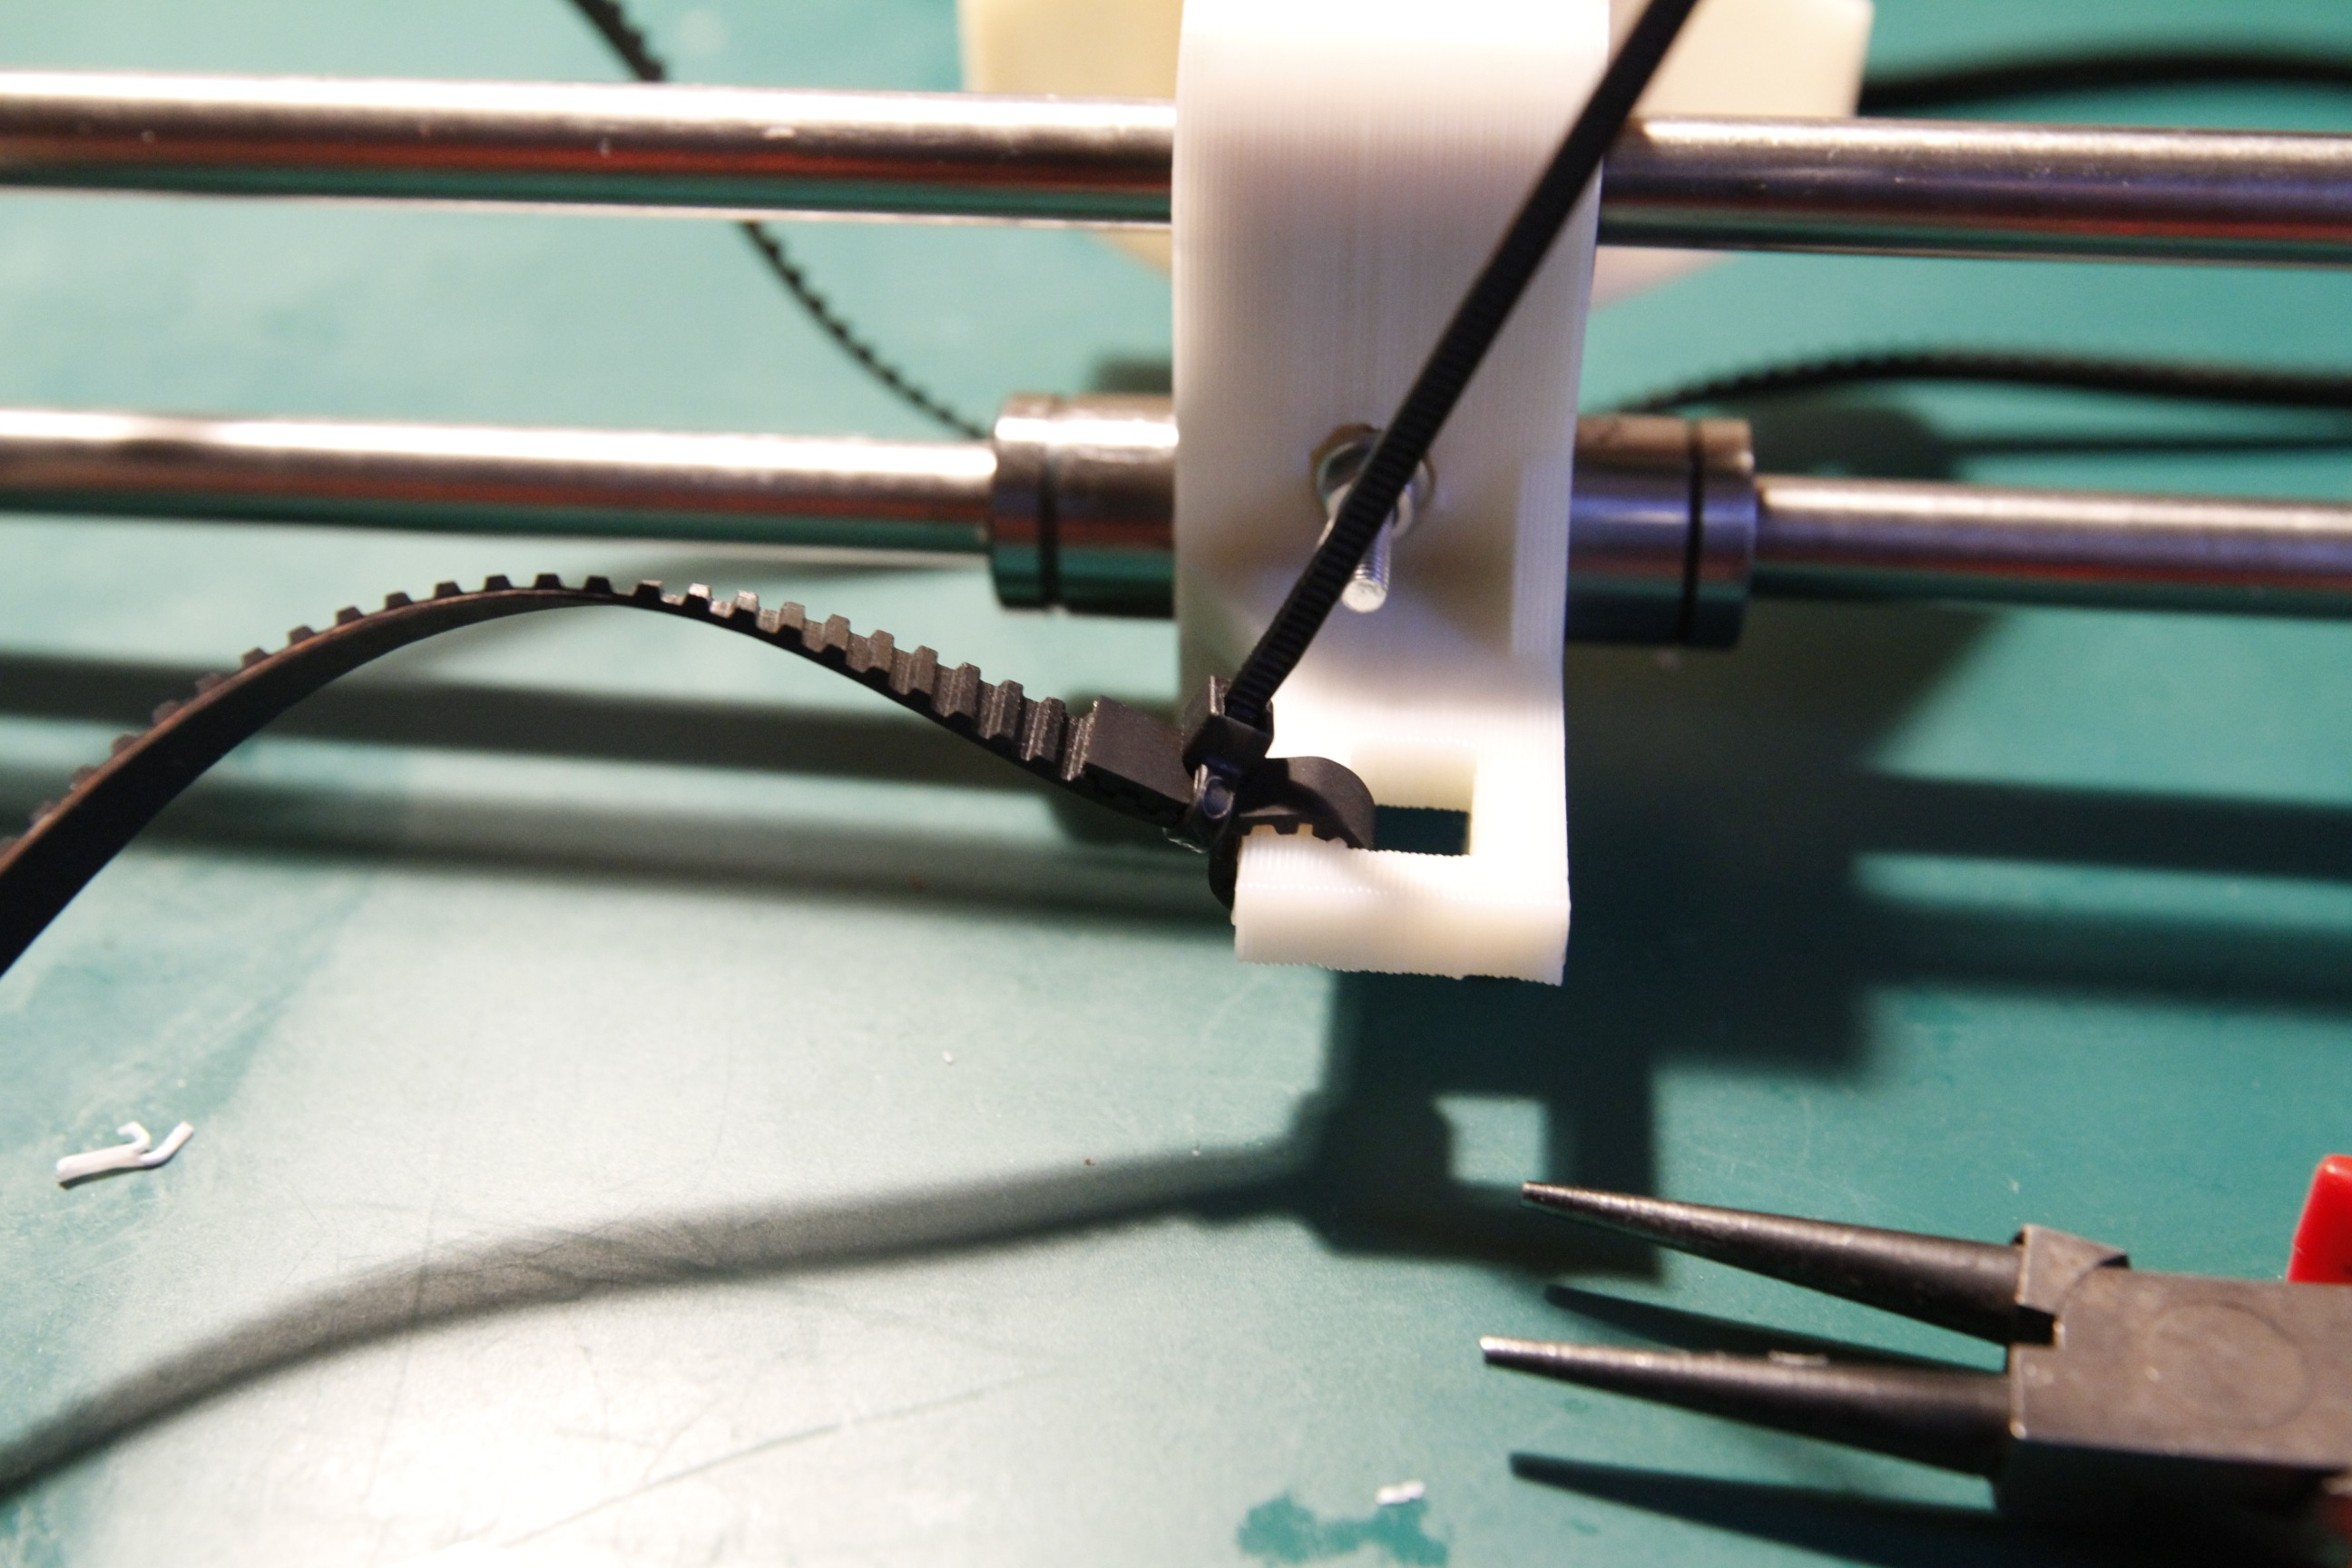
\includegraphics[width=0.6\textwidth]{../../Fotos/65.jpg}
				\caption{Correa eje X}
				%\label{fig:motor.ejex}
			\end{figure}
			Para finalizar con el eje X, instalamos el endstop en en la pieza donde va colocado el motor.\\
			\begin{figure}[!htp]
				\centering
				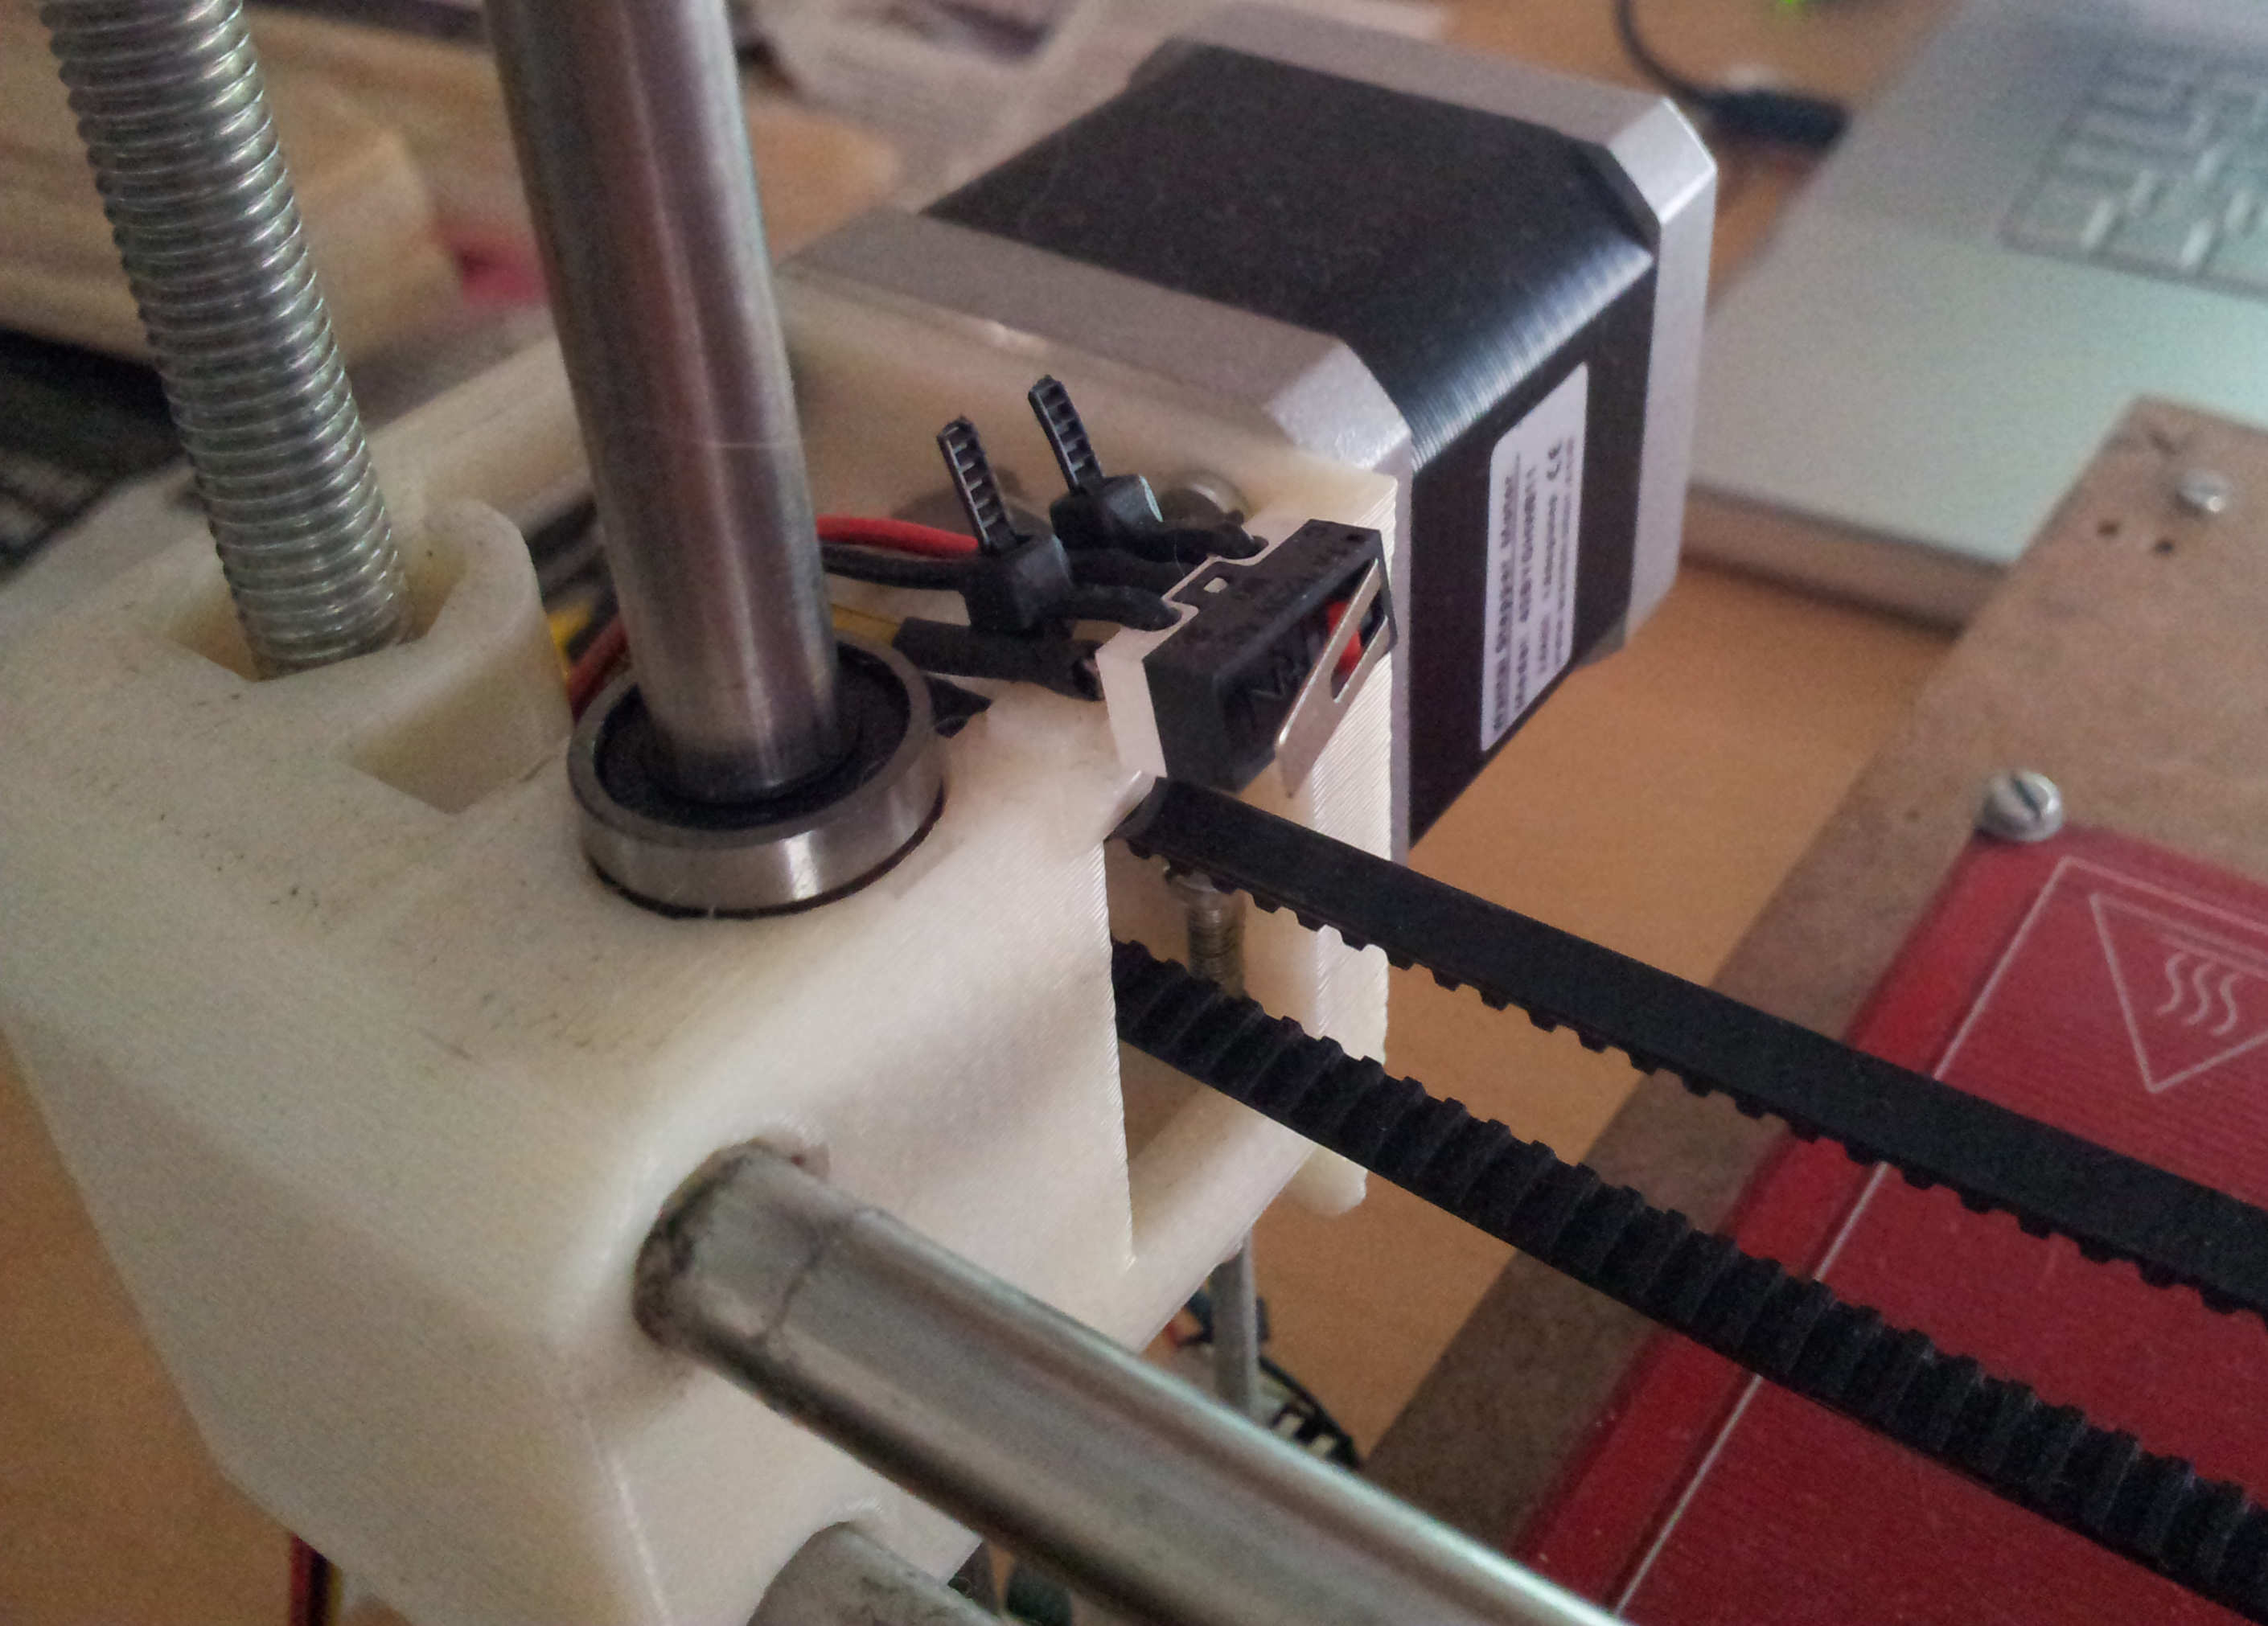
\includegraphics[width=0.5\textwidth]{../../Fotos/66.jpg}
				\caption{Conjunto Extrusor}
				%\label{fig:motor.ejex}
			\end{figure}
			En caso de disponer de unos endstop pequeños, es recomendable usar una pieza auxiliar como se muestra en la figura ~\ref{fig:1.ejex}
			\begin{figure}[!htp]
				\centering
				\includegraphics[width=0.5\textwidth]{../../Fotos/109.jpg}
				\caption{Micro Endstop }
				\label{fig:1.ejex}
			\end{figure}
			La colocación en la impresora es de forma análoga que en la impresora Prusa Mendel(~\ref{fig:2.ejex}). Es recomendable hacer esta operación con los endstop del eje X y Z.\\
			\begin{figure}[!htp]
				\centering
				\includegraphics[width=0.5\textwidth]{../../Fotos/110.jpg}
				\caption{Instalación micro-endstop}
				\label{fig:2.ejex}
			\end{figure}